% Options for packages loaded elsewhere
\PassOptionsToPackage{unicode}{hyperref}
\PassOptionsToPackage{hyphens}{url}
%
\documentclass[
]{article}
\usepackage{amsmath,amssymb}
\usepackage{iftex}
\ifPDFTeX
  \usepackage[T1]{fontenc}
  \usepackage[utf8]{inputenc}
  \usepackage{textcomp} % provide euro and other symbols
\else % if luatex or xetex
  \usepackage{unicode-math} % this also loads fontspec
  \defaultfontfeatures{Scale=MatchLowercase}
  \defaultfontfeatures[\rmfamily]{Ligatures=TeX,Scale=1}
\fi
\usepackage{lmodern}
\ifPDFTeX\else
  % xetex/luatex font selection
\fi
% Use upquote if available, for straight quotes in verbatim environments
\IfFileExists{upquote.sty}{\usepackage{upquote}}{}
\IfFileExists{microtype.sty}{% use microtype if available
  \usepackage[]{microtype}
  \UseMicrotypeSet[protrusion]{basicmath} % disable protrusion for tt fonts
}{}
\makeatletter
\@ifundefined{KOMAClassName}{% if non-KOMA class
  \IfFileExists{parskip.sty}{%
    \usepackage{parskip}
  }{% else
    \setlength{\parindent}{0pt}
    \setlength{\parskip}{6pt plus 2pt minus 1pt}}
}{% if KOMA class
  \KOMAoptions{parskip=half}}
\makeatother
\usepackage{xcolor}
\usepackage[margin=1in]{geometry}
\usepackage{graphicx}
\makeatletter
\newsavebox\pandoc@box
\newcommand*\pandocbounded[1]{% scales image to fit in text height/width
  \sbox\pandoc@box{#1}%
  \Gscale@div\@tempa{\textheight}{\dimexpr\ht\pandoc@box+\dp\pandoc@box\relax}%
  \Gscale@div\@tempb{\linewidth}{\wd\pandoc@box}%
  \ifdim\@tempb\p@<\@tempa\p@\let\@tempa\@tempb\fi% select the smaller of both
  \ifdim\@tempa\p@<\p@\scalebox{\@tempa}{\usebox\pandoc@box}%
  \else\usebox{\pandoc@box}%
  \fi%
}
% Set default figure placement to htbp
\def\fps@figure{htbp}
\makeatother
\setlength{\emergencystretch}{3em} % prevent overfull lines
\providecommand{\tightlist}{%
  \setlength{\itemsep}{0pt}\setlength{\parskip}{0pt}}
\setcounter{secnumdepth}{-\maxdimen} % remove section numbering
% definitions for citeproc citations
\NewDocumentCommand\citeproctext{}{}
\NewDocumentCommand\citeproc{mm}{%
  \begingroup\def\citeproctext{#2}\cite{#1}\endgroup}
\makeatletter
 % allow citations to break across lines
 \let\@cite@ofmt\@firstofone
 % avoid brackets around text for \cite:
 \def\@biblabel#1{}
 \def\@cite#1#2{{#1\if@tempswa , #2\fi}}
\makeatother
\newlength{\cslhangindent}
\setlength{\cslhangindent}{1.5em}
\newlength{\csllabelwidth}
\setlength{\csllabelwidth}{3em}
\newenvironment{CSLReferences}[2] % #1 hanging-indent, #2 entry-spacing
 {\begin{list}{}{%
  \setlength{\itemindent}{0pt}
  \setlength{\leftmargin}{0pt}
  \setlength{\parsep}{0pt}
  % turn on hanging indent if param 1 is 1
  \ifodd #1
   \setlength{\leftmargin}{\cslhangindent}
   \setlength{\itemindent}{-1\cslhangindent}
  \fi
  % set entry spacing
  \setlength{\itemsep}{#2\baselineskip}}}
 {\end{list}}
\usepackage{calc}
\newcommand{\CSLBlock}[1]{\hfill\break\parbox[t]{\linewidth}{\strut\ignorespaces#1\strut}}
\newcommand{\CSLLeftMargin}[1]{\parbox[t]{\csllabelwidth}{\strut#1\strut}}
\newcommand{\CSLRightInline}[1]{\parbox[t]{\linewidth - \csllabelwidth}{\strut#1\strut}}
\newcommand{\CSLIndent}[1]{\hspace{\cslhangindent}#1}
\usepackage{titling}
\usepackage{booktabs}
\usepackage{pdflscape}
\usepackage{pgfplots}
\usepackage{tikz}
\usetikzlibrary{positioning, arrows, shapes.geometric}
\usepackage[dvipsnames, table]{xcolor}
\usepackage{lscape}
\usepackage{float}
\usepackage{amsmath}
\usepackage{fancyhdr}
\usepackage{caption}
\captionsetup[figure]{labelformat=empty}
\captionsetup[table]{labelformat=empty}
\usepackage{etoolbox}
\fancyhf{}
\rfoot{\thepage}
\pagenumbering{gobble}
\pretitle{\begin{center}\LARGE}
\posttitle{\par\end{center}}
\preauthor{\begin{center}\large}
\postauthor{\par\end{center}}
\predate{\begin{center}\small}
\usepackage{booktabs}
\usepackage{longtable}
\usepackage{array}
\usepackage{multirow}
\usepackage{wrapfig}
\usepackage{float}
\usepackage{colortbl}
\usepackage{pdflscape}
\usepackage{tabu}
\usepackage{threeparttable}
\usepackage{threeparttablex}
\usepackage[normalem]{ulem}
\usepackage{makecell}
\usepackage{xcolor}
\usepackage{tabularray}
\usepackage[normalem]{ulem}
\usepackage{graphicx}
\usepackage{rotating}
\UseTblrLibrary{booktabs}
\UseTblrLibrary{siunitx}
\NewTableCommand{\tinytableDefineColor}[3]{\definecolor{#1}{#2}{#3}}
\newcommand{\tinytableTabularrayUnderline}[1]{\underline{#1}}
\newcommand{\tinytableTabularrayStrikeout}[1]{\sout{#1}}
\usepackage{bookmark}
\IfFileExists{xurl.sty}{\usepackage{xurl}}{} % add URL line breaks if available
\urlstyle{same}
\hypersetup{
  pdftitle={Cold Calculations - How Conflict Characteristics Shape External Support in Armed Conflicts},
  pdfauthor={Celine Giese and Thiago R. Oliveira},
  hidelinks,
  pdfcreator={LaTeX via pandoc}}

\title{Cold Calculations - How Conflict Characteristics Shape External
Support in Armed Conflicts}
\author{Celine Giese and Thiago R. Oliveira}
\date{}

\begin{document}
\maketitle

{
\setcounter{tocdepth}{2}
\tableofcontents
}
\newpage

\section{Table of Figures}\label{table-of-figures}

\begin{center}
\begin{tabular}{l l r}
\textbf{Type} & \textbf{Title} & \textbf{Page} \\

\\[-0.3em]
\multicolumn{3}{l}{\textbf{Tables}} \\[0.3em]
Table 1 & Variables used in the analysis & 13 \\
Table 2 & Regression Results – External Support Determinants & 20 \\
Table 3 & Statistical Significance in the RE and FE Logistic Regression Models & 21 \\
Table 4 & RE and FE Logistic and PPML Regression Results & 24 \\[1.2em]

\multicolumn{3}{l}{\textbf{Figures}} \\[0.3em]
Figure 1 & Directed Acyclic Graph on Conflict Characteristics and External Support & 10 \\
Figure 2 & World armed conflicts by intensity level & 18 \\[0.3em]
Figure 3 & Mean and Median Conflict Duration by Region & 18 \\
Figure 4 & Direct and Indirect Support, 1975–2017 & 19 \\[1.2em]

\multicolumn{3}{l}{\textbf{Appendices}} \\[0.3em]
Appendix 1 & State-based Conflicts by Region, 1975–2017 & 26 \\
Appendix 2 & State-based Conflicts by Type of Conflict, 1975–2017 & 26 \\
Appendix 3 & Conflict Type by Region & 27 \\
Appendix 4 & Evolution of State-based Conflicts by Incompatibility, 1975–2017 & 27 \\
Appendix 5 & Evolution of External Support: Bilateral vs Coalition & 28 \\
Appendix 6 & Statistical Significance in the RE Linear Regression models & 29 \\

\end{tabular}
\end{center}

\newpage

\section{Data availability statement}\label{data-availability-statement}

All analyses were conducted in R (R Core Team (2025)), with the analytic
code and input data made publicly available on
\href{https://github.com/celine-felicit/Dissertation-Code}{GitHub} to
ensure transparency and facilitate replication.

\section{Abstract}\label{abstract}

Armed conflicts shape not only military but also social priorities,
often diverting resources from social welfare to defence (Sivard
(1996)). Their consequences can be devastating and long-lasting,
affecting economic development, social structures, and state stability.
As contemporary conflicts continue to unfold globally, understanding how
and why states choose to intervene - particularly through external
support (ES) - is increasingly relevant. Such interventions raise
critical questions about international responsibility and complicity,
especially when support facilitates war crimes. Despite this, armed
conflict has received limited attention within Criminology. This study
seeks to address that gap by investigating whether and how conflict
characteristics influence the provision and form of ES. Drawing on 472
dyads in 212 conflicts between 1975 and 2017, sourced from the Uppsala
Conflict Data Program (UCDP), the analysis is guided by a Directed
Acyclic Graph (DAG) that maps assumed causal pathways. The study employs
within-between logistic regression models to test hypotheses on the
influence of conflict characteristics - such as intensity, duration, and
type - on the provision of ES, including whether support is given
bilaterally or through coalitions. Based in criminological research on
violence (Collins (2008)) this suggests a ``cold'' approach to the
provision of external support, where external supporters consider the
conflict dynamics before providing support. This research contributes to
a more comprehensive understanding of the interplay between external
interventions and conflict dynamics, bridging critical gaps in
criminology and offering a starting point for criminological discussion
around the liability and responsibility of external supporters.

\newpage

\section{Introduction}\label{introduction}

Despite a reduction in conflicts and deaths, the past decade remains the
most violent on record (Davies et al. (2024)). War and armed conflicts
(AC) profoundly impact parties involved, with ordinary civilians
disproportionately suffering due to fatalities, displacement, and
long-term public health crises from destroyed infrastructure (Hoeffler
and Reynal-Querol (2003)). War-torn countries face reduced growth,
higher poverty rates, and weakened institutions, with recovery dependent
on robust policy reforms (Hoeffler and Reynal-Querol (2003)).
High-intensity violence during conflicts lowers economic growth, life
expectancy, and educational attainment, with these effects often
persisting long-term (Le et al. (2022)). Wars and ACs further generate
significant spillover effects, with severity influenced by geographic
proximity and economic ties to the conflict zone. Neighbouring countries
often face adverse economic consequences, while distant nations
experience milder effects due to limited trade links and geographic
distance (Federle et al. (2024)). Regions with stronger economic ties to
the conflict zone experience amplified negative impacts, including
disrupted stability and heightened uncertainty (Fang et al. (2020); Le
et al. (2022)). While inflation and output remain stable in distant
countries, the ripple effects of war challenge interconnected global
economies, highlighting the complex dynamics between conflict and
economic stability (Federle et al. (2024)). The enduring economic and
social costs of war underscore its profoundly criminogenic nature.

Today, although conflicts are largely fought by developing nations, they
rely heavily on advanced military equipment produced by industrial
countries, reinforcing military over social investments (Sivard (1996)).
The prevalence and complexity of external support (ES) in AC have grown
significantly over the past decades. From 1975 to 2017, 80\% of
intrastate conflicts involved at least one instance of ES, with state
actors being the predominant supporters (Meier et al. (2023)). Recent
years have seen systemic shifts in ES, characterised by the rise of
multilateral coalitions and collaborative interventions. Nearly
one-third of all support instances now involve such coalitions,
emphasising burden-sharing and the legitimacy of support (Meier et al.
(2023)). However, recent developments, such as the United States cutting
off significant amounts of its financial and military support for
Ukraine, and humanitarian aid to Syria (Sandefur and Kenny (2025); UN
(2025)), cast doubt on the future of military alliances and joint
defence initiatives like the North Atlantic Treaty Organisation (NATO),
as well as the accountability and durability of assistance. With many
geopolitical tensions and conflicts ongoing, discussions around AC and
ES are crucial to the political environment and international relations,
raising questions around the responsibility and accountability of
external supporters, especially when military actions turn into war
crimes.

While an extremely timely topic, Criminology has historically neglected
AC (Hagan (2015); Jamieson (2003); Ruggiero (2015); McGarry and Walklate
(2015)), let alone ES. But even in research on ES, the content of
interventions remains underexplored, despite its impact on conflict
trajectories (see for example Cunningham (2016); Karlén (2017); Aydin
and Regan (2012)). This research adopts an interdisciplinary approach,
integrating Criminology, Peace and Conflict Studies, and Economics to
examine whether conflict characteristics affect the provision of ES and
identify trends and conditions under which ES is provided. While
Economics tend to focus on the economic costs of conflicts, using
quantitative analysis to analyse the economic effects and spillover of
conflicts (see for example (Federle et al. (2024); Fang et al. (2020);
Sivard (1996)), Peace and Conflict studies predominantly use qualitative
approaches, focusing on the prevention, resolution, and transformation
of conflict (i.e.~\emph{INSERT REFERENCE}). Critical Criminology, which
has started to engage with AC primarily does so from a theoretical
and/or qualitative approach, predominantly focusing on the criminogenic
nature of war as a whole (i.e. Ruggiero (2005)) and genocide (i.e.
Rafter (2016)). Through drawing on literature from Economics, as well as
Peace and Conflict studies, this study aims to combine the quantitative
approach of Economics with the focus areas of Peace and Conflict studies
and criminological theories to offer broader insights into the areas of
ES and AC. By distinguishing between support types, it further aims to
provide a more robust understanding of the role of external supporters
and their motives, essential for further discussions around liability
and responsibility. In doing so, it bridges critical gaps in
Criminology, contributing to a more comprehensive understanding of the
interplay between external interventions and conflict dynamics.

This study addresses three research questions: (1) Do conflict
characteristics influence the provision of ES? (2) Do they affect the
form of support provided? (3) Does coalition-based support influence
what type of support is provided? The data comes from two Uppsala
Conflict Data Program (UCDP) datasets: the Dyadic Dataset (Version
18.1), covering conflict characteristics between 1946 and 2018 (Harbom
et al. (2008); Pettersson and Eck (2018)), and the External Support
Dataset (Version 18.1), which captures ten forms of ES between 1975 and
2017 (Meier et al. (2023)). The high-quality data produced by UCDP is
methodically gathered, covers mass violence globally, and includes
long-term series that are updated once a year. It is the oldest civil
war data collection and allows for comparisons between conflicts and
nations. Its definition of AC has evolved into the accepted worldwide
norm for the methodical definition and analysis of conflicts. Together,
the two datasets provide a robust foundation for quantitatively
analysing the relationship between conflict characteristics and ES. To
answer the research questions, the study uses within-between logistic
regression models, allowing for the examination of both within- and
between-dyad variation. These methods are well suited to the dyadic
nature of AC data and support the identification of strategic patterns
in support provision---insights essential for discussions on the
liability and responsibility of external actors. Therefore, this study
contributes to a more nuanced understanding of the interplay between
external interventions and conflict dynamics, addressing critical gaps
in criminological literature on accountability in AC. The study is
structured as follows: First, existing literature on AC and ES is
reviewed, highlighting gaps in criminological scholarship and
introducing the conceptual lens of `hot' versus `cold' mass violence.
The research design and theoretical framework are then described,
followed by the methodology, data, and operationalisation. Following the
presentation of the findings, it finishes with the discussion and
concluding reflections.

\section{Literature Review}\label{literature-review}

The landscape of AC has shifted in recent decades, with a rise in
internationalised intrastate conflicts where external states support
non-state actors opposing governments (Davies et al. (2024)). This study
uses the UCDP's definition of AC, which has become a norm for the
methodical definition and analysis of conflicts. AC herein is defined as
`a contested incompatibility that concerns government and/or territory
where the use of armed force between two parties, of which at least one
is the government of a state, results in at least 25 battle-related
deaths in a calendar year' (Themnér (2018), p.2). The primary parties in
such conflicts include governments, which control the state capital, and
opposition organisations, which are formally organised groups using
armed force to influence the outcome of the incompatibility.

Although developing nations fight most of today's conflicts, they are
often fought with weapons from industrialised countries, reflecting
20th-century technological advancements (Sivard (1996)). As geopolitical
tensions rise, the role of ES in these conflicts has become a central
topic of discussion (Federle et al. (2024)). ES, defined as militarily
relevant assistance provided by outside parties to active conflicts, is
distinct from peacetime activities like arms trade or security reforms
(Meier et al. (2023); Meier (2022)). This support aims to enhance the
recipient's military capabilities and is provided with the clear intent
of facilitating military victory over the opposing side (Cunningham
(2010); Gregory (2000)). It includes materiel, knowledge, or services
directly aiding warfare but excludes unintentional support like
sanctions that weakens a conflict party but is not intended to support
the other side. Additionally, diplomatic efforts, humanitarian aid, and
mediation offers do not qualify as ES since they do not directly
contribute to the military outcome (Meier (2022)). The external nature
of support is determined by whether the provider is not a primary
warring party in the conflict, even if present in the same territory.

The interplay between conflict characteristics and ES is complex, with
interventions - whether direct military actions or indirect aid - often
prolonging hostilities and complicating peace efforts (Sawyer et al.
(2015); Karlén (2023); Regan (2002)). Understanding why and how states
intervene and the consequences of different types of support is vital to
analysing external involvement. This research seeks to explore these
themes, examining how conflict characteristics shape external
interventions.

\subsection{The study of armed conflicts in
Criminology}\label{the-study-of-armed-conflicts-in-criminology}

Following the so-called `century of peace' (1815--1914), war has
continued across regions, yet social sciences have failed to reflect its
prevalence or significance. States, through their `legitimate monopoly
of violence' (Weber (1919) in McGarry and Walklate (2019)), justify
violence via bureaucratic rationality, framing war as a noble endeavour
to solidify authority and autonomy (Malešević (2010) in Walklate and
McGarry (2019)). Historically, war was driven by imperial capitalist
expansion, which fuels conflicts through profit-driven globalisation
(Ruggiero (2023); Bonger (1916) in Walklate and McGarry (2019); Klein
(2011)). Even today, economic imperatives often guide responses to war,
reducing it to a developmental obstacle. The global capitalist system
blurs lines between legitimate but harmful actions, exacerbating
violence (Ruggiero (2005)). Critical criminologists therefore view war
as a form of state crime legitimised by dominant powers who shape
international norms to justify past and future conflicts (Kramer and
Michalowski (2005); Bonanate (2011) in Ruggiero (2023)). Despite
millions of legitimate killings in war, criminology has been reluctant
to challenge the legitimacy of such violence or address its broader
systemic causes (Ruggiero (2005)). Wartime atrocities are reframed as
patriotic acts, aligning with state narratives through techniques of
neutralisation (Sykes and Matza (1957); Ruggiero (2005)). These dynamics
underscore the importance of rethinking state authority, as legality and
illegality are often strategically maneuvered in the pursuit of power
(Heyman (1999) in Ruggiero (2005)). Criminologists, long defining crime
not only over illegality but over harm (Hillyard and Tombs (2007)), have
a unique opportunity to address its multifaceted impacts and advocate
for systemic reforms (Jamieson (1998) in McGarry et al. (2016); Ruggiero
(2005)). Due to its central role to conflicts, examining ES is essential
to understanding underlying dynamics of AC. It further raises critical
questions about complicity and liability for war crimes, and whether ES
escalates violence or fosters peace.

To examine the dynamics of ES, offering insights into the motives and
strategies of external intervention, this study analyses ES through the
lens of `hot' and `cold' conflicts, a principle first developed by
Collins (Collins (2008)). According to Collins (2008) in (Rafter (2016),
p.98), whether fighting actually breaks out in violent confrontations
between individuals or groups depends on `a series of conditions or
turning-points that shape the tension and fear in particular directions,
reorganising the emotions as an interactional process involving everyone
present: the antagonists, audience, and even ostensibly disengaged
bystanders'. These turning points operate as triggers for later (but
still contingent) behaviours and signal a break with the feelings of the
past. Criminological studies on mass violence (MV) have looked at the
situational dynamics of such acts, distinguishing between `hot' and
`cold' acts of MV (Rafter (2016)), reflecting their underlying emotional
dynamics. At the core of `hot' MV is the notion of `forward panic' - a
form of violence that emerges when prolonged fear and tension build up,
then suddenly discharge in a wave of uncontrolled aggression. This
pattern is marked by emotional entrainment: participants get caught in a
rhythm of escalating violence that feels unstoppable in the moment
(Collins (2008)). Emotions such as rage, fear, elation, and a sense of
moral detachment combine to create a state of high physiological and
social arousal. In contrast, `cold' violence is premeditated, detached,
and bureaucratised. It reflects deliberate planning and instrumental
logic, often implemented through structures of command or strategy.
While it lacks the overt emotional frenzy of forward panics, it is no
less violent - merely more strategic, procedural, and distanced from
immediate confrontation. These categories are not mutually exclusive:
conflicts may shift between `hot' and `cold' phases or contain elements
of both. Importantly, Collins (2008) theory treats emotional dynamics
not as irrational noise but as socially organised processes with
identifiable triggers and consequences. Applying this lens to the
provision of ES, this study hypothesises that external supporters -
distant from the emotional immediacy of the battlefield - act more in
line with `cold' violence logics. Support decisions are hypothesised to
reflect calculated responses to conflict characteristics such as
intensity, duration, type, or geopolitical timing (e.g., post-9/11). By
testing whether certain conflict characteristics are correlated with the
overall provision and type of ES, the study examines whether ES is best
understood as a strategic, interest-driven act rather than an
emotionally reactive one.

\subsection{External support to armed
conflicts}\label{external-support-to-armed-conflicts}

Despite only a slight rise in total conflicts over recent decades, the
number of actors providing ES has grown(Meier et al. (2023)). While
troop support has declined, the total number of external interventions
continues to grow, reflecting persistent interest in shaping conflict
trajectories through both direct and indirect means (Davies et al.
(2024); Chang and Sellak (2022)). By 2017, 77\% of active conflict-dyads
featured state support for governments alone, driven in part by the
post-9/11 counter terrorism focus, which stigmatised support for
non-state actors (Meier et al. (2023)). Multilateral counter-extremism
efforts, often led by UN Security Council members, have reinforced this
trend (Meier et al. (2023)). Research on ES in ACs highlights its
significant impact on conflict dynamics and outcomes. The provision of
ES shapes the onset (Cunningham (2016); Regan and Meachum (2014)),
duration (Aydin and Regan (2012); Anderson (2019)), outcomes (Sawyer et
al. (2015)), and recurrence (Karlén (2017)) of ACs. Interventions,
whether direct (troops) or indirect (weapons, logistics, training),
frequently prolong conflicts by altering the cost-benefit calculations
of belligerents (Fearon (2004) in Testerman (2015); Lacina (2006)) and
although external aid can alter power dynamics, it frequently
intensifies conflicts, complicates negotiations, and reduces the
likelihood of peaceful resolutions (Olson Lounsbery (2016); Zartman
(1992) in Saideman (2002); Salehyan et al. (2011); Petrova (2019)).
Although ES can improve the odds of military victory (Balch-Lindsay et
al. (2008)), it often exacerbates humanitarian crises, with rebels
exploiting moral hazards to attract further intervention (Rauchhaus
(2009); Karlén (2017)). Overall, external actors, including state and
non-state supporters, play pivotal roles by shaping conflict processes
through diverse forms of assistance, such as military training and
direct intervention (Gleditsch (2007); Salehyan (2010); Toukan (2019)).

The type and target of ES often align with intervening parties'
strategic interests. While training and expertise remain the most
frequent forms of support, material aid dominates assistance to rebel
groups (Meier et al. (2023); Berlin and Malone (2023)), suggesting that
the type of ES provided differs based on the recipients. Support
dynamics further vary by conflict intensity, geographic proximity, and
the relative strength of involved parties (Goldman and Abulof (2016);
Meulewaeter (2021); Olson Lounsbery (2016); Salehyan et al. (2011)). The
Cold War intensified conflicts through superpower support, but its end
shifted patterns, reducing insurgencies and prolongation, while rebel
groups lost aid, leading many conflicts to peter out or end in
settlements (Testerman (2015); Kalyvas and Balcells (2010) in Roberts
(2019)). While previous studies have established correlations between
characteristics of conflicts and conflict parties, and quite a few have
done so using data from the UCDP (Meulewaeter (2021); Salehyan et al.
(2011); Olson Lounsbery (2016); Testerman (2015); Karlén (2017); Le et
al. (2022)), most analysed the correlation between only one or two
conflict characteristics and ES. Most studies further focus on the
economic and social cost of conflict (e.g. Federle et al. (2024);
Testerman (2015); Le et al. (2022); Sivard (1996)), or on the effects of
ES on conflict dynamics, rather than the provision of ES itself. The
introduction of the UCDP ESD (Meier et al. (2023)) offers an extensive
descriptive overview of ES dynamics and an opportunity for extensive
quantitative analysis of ES, making it easier to research ES dynamics.
However, questions as to when, why, and how states are likely to
intervene remain to be researched.

Previous research shows that external supporters engage in civil
conflicts for diverse and strategic reasons, including geopolitical,
economic, and ideological motives, as well as specific foreign policy
objectives (Findley and Teo (2006); Meier et al. (2023)). Economic
interests often drive involvement, with external powers seeking to
protect trade benefits or access resources by backing domestic victors
(Regan (1998); Kathman (2011)). In some instances, involvement appears
benevolent, such as facilitating peace talks (Bhattarai (2016)).
However, third-party intervention is rarely altruistic; states often aim
to weaken adversaries, prevent conflict spillover, or maintain influence
in post-colonial regions (Cunningham (2010); Gregory (2000)).
Strategically, sponsoring militant groups enables states to destabilise
rivals or gain leverage without direct conflict. Delegating violence
minimises costs while exploiting the instability inflicted on
adversaries (Schultz (2010); Bapat (2012)). However, this approach
carries risks, including retaliation, escalation, and the possibility
that armed groups will pursue independent agendas (Schultz (2010); Maoz
and San-Akca (2012)). Shared ethnic or ideological ties between sponsors
and armed groups signal shared goals and reduce the risk that resources
will be misused (Berlin and Malone (2023); Salehyan (2010)). They are
therefore among the strongest predictors of ES (Salehyan et al. (2011);
Sozer (2016)), as they further facilitate communication and enhance
trust, improving cooperation (San-Akca (2016); Bacon (2018)). However,
relying on such ties can oversimplify sponsorship decisions, especially
in contexts with multiple potential recipients or competing priorities
(Berlin and Malone (2023)). Ultimately, prior research suggests that ES
is a calculated foreign policy tool used to influence conflict outcomes
while advancing sponsors' strategic goals.

\subsubsection{Limitations of past
research}\label{limitations-of-past-research}

The study of ES in ACs has provided critical insights but is hindered by
several limitations. Much research focuses predominantly on support for
non-state armed groups, particularly rebel organisations, sidelining
other actors and minor armed engagements (Walter (2004); Quinn et al.
(2007); Salehyan et al. (2011)). A focus on rebel groups introduces
methodological challenges and selection bias, limiting generalisability
to other armed organisations (Abrahms et al. (2018); Phillips (2019)).
This neglect obscures patterns of ES across diverse settings,
undermining frameworks linking organisational attributes to state
sponsorship. Furthermore, the multi-actor dimension of support is
frequently overlooked, despite evidence that sponsors selectively
support specific groups within fragmented conflicts (Berlin and Malone
(2023)). Studies often emphasise the initial decision to delegate
support (Salehyan (2010); San-Akca (2016)), neglecting how support
dynamics evolve throughout a conflict's lifecycle and the strategic
factors influencing its continuation or cessation (Karlén (2019);
Tokdemir et al. (2021)). The content of interventions remains
underexplored, despite its impact on conflict trajectories.
Differentiating between support types - military training, material aid,
or safe havens - can highlight distinct effects on outcomes (Roberts
(2019)). Moreover, qualitative approaches dominate the literature, often
at the expense of quantitative or mixed method analyses better suited to
capturing temporal and contextual variations in support dynamics
(Petrova (2019)). This research addresses these limitations by examining
the interplay between conflict characteristics and different types of ES
from a quantitative criminological angle, aiming to provide a starting
point for further criminological discussions around the liability and
responsibility of external supporters in ACs. By analysing trends in ES
provision both within and between conflict-dyads, it further builds on
previous research, offering a more nuanced understanding of the
strategic factors influencing ES.

\begin{landscape}
\begin{figure}[htbp!]
\centering

\resizebox{1.1\linewidth}{!}{%
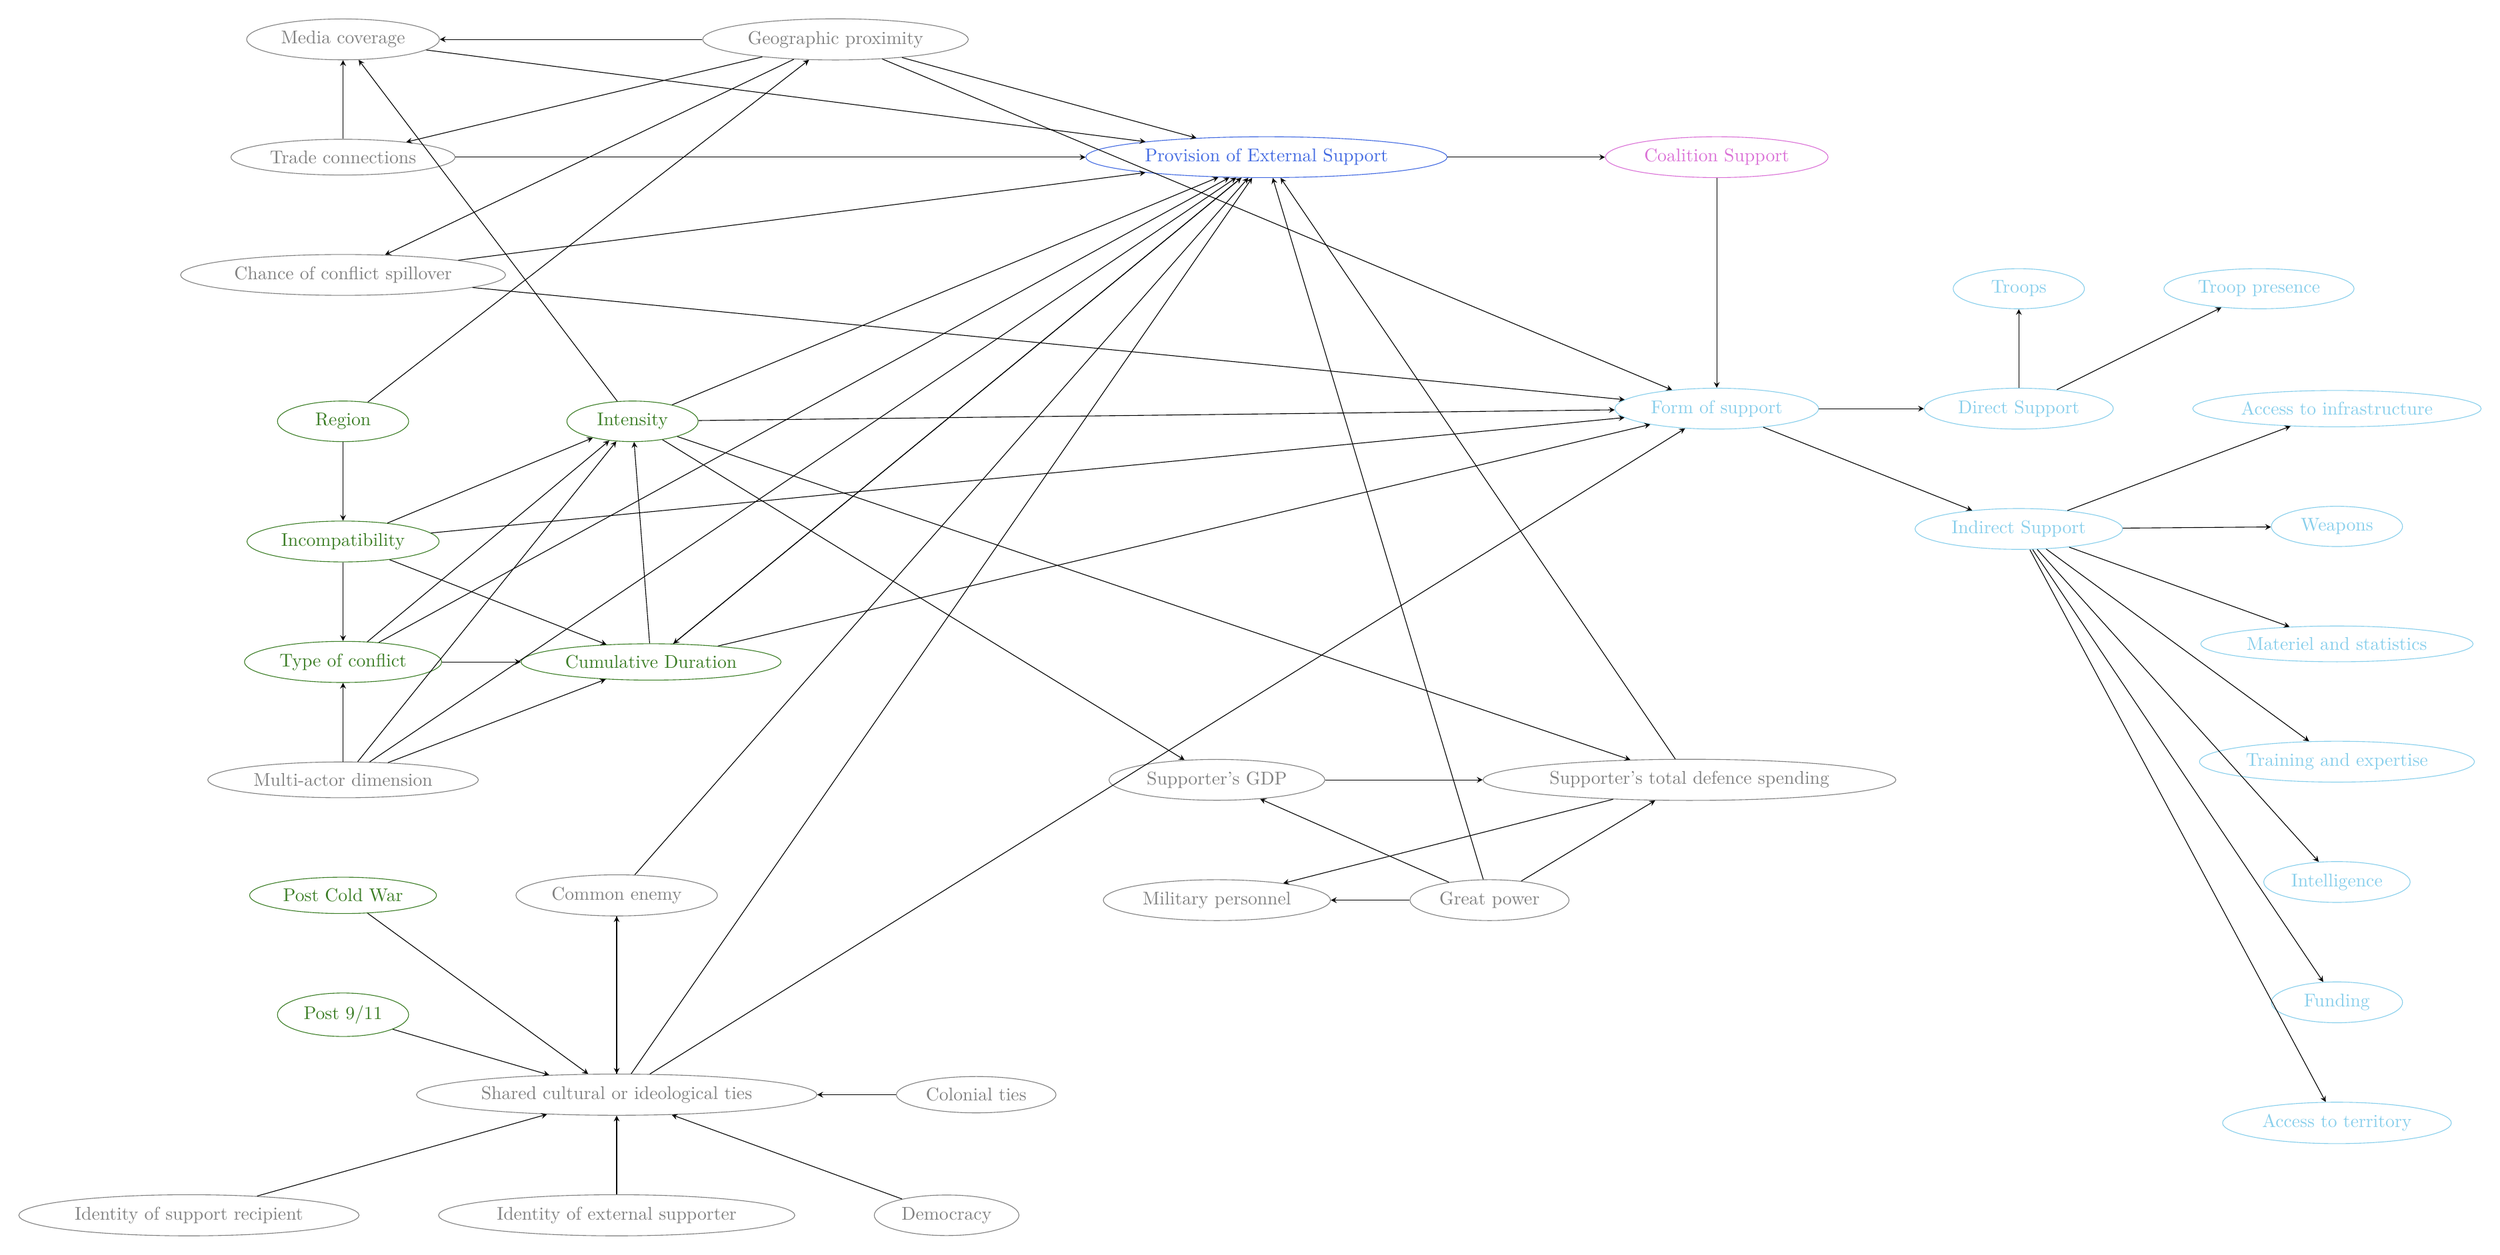
\begin{tikzpicture}[
  scale=1, 
  every node/.style={draw, ellipse, align=center, minimum width=2.5cm}, 
  node distance=1.5cm, 
  ->, >=stealth
]

% Conflict Characteristics and control variables
\node[color = OliveGreen] (incompatibility) {Incompatibility};
\node[below=of incompatibility, color = OliveGreen] (type) {Type of conflict};
\node[above=of incompatibility, color = OliveGreen] (region) {Region};
\node[right=3cm of region, color = OliveGreen] (intensity) {Intensity};
\node[below=of type, color = Gray] (multiactor) {Multi-actor dimension};
\node[right=of type, color = OliveGreen] (duration) {Cumulative Duration};
\node[below=of multiactor, color = OliveGreen] (coldwar) {Post Cold War};
\node[below=of coldwar, color = OliveGreen] (nineeleven) {Post 9/11};
\node[right=of coldwar, color = Gray] (enemy) {Common enemy};
\node[below=3cm of enemy, color = Gray] (culturalties) {Shared cultural or ideological ties};
\node[below=of culturalties, color = Gray] (identityes) {Identity of external supporter};
\node[left=of identityes, color = Gray] (identityrec) {Identity of support recipient};
\node[right=of culturalties, color = Gray] (colonial) {Colonial ties};
\node[right=of identityes, color = Gray] (democracy) {Democracy};

\node[above=2cm of region, color = Gray] (spillover) {Chance of conflict spillover};
\node[above=of spillover, color = Gray] (trade) {Trade connections};
\node[above=of trade, color = Gray] (media) {Media coverage};
\node[right=5cm of media, color = gray] (geography) {Geographic proximity};

\node[right=12cm of multiactor, color = Gray] (GDP) {Supporter's GDP};
    \node[right=3cm of GDP, color = Gray] (defence) {Supporter's total defence spending};
\node[below=of GDP, color = Gray] (military) {Military personnel};
\node[right=of military, color = Gray] (greatpower) {Great power};

% External Support
\node[right=12cm of trade, color = RoyalBlue] (external) {Provision of External Support};
\node[right=3cm of external, color = Orchid] (coalition) {Coalition Support};
\node[below=4cm of coalition, color = SkyBlue] (form) {Form of support};
\node[right=2cm of form, color = SkyBlue] (direct) {Direct Support};
\node[below=of direct, color = SkyBlue] (indirect) {Indirect Support};
\node[above=of direct, color = SkyBlue] (troops) {Troops};
\node[right=of troops, color = SkyBlue] (presence) {Troop presence};
\node[right=of direct, color = SkyBlue] (infrastructure) {Access to infrastructure};
\node[below=of infrastructure, color = SkyBlue] (weapons) {Weapons};
\node[below=of weapons, color = SkyBlue] (logistics) {Materiel and statistics};
\node[below=of logistics, color = SkyBlue] (training) {Training and expertise};
\node[below=of training, color = SkyBlue] (intelligence) {Intelligence};
\node[below=of intelligence, color = SkyBlue] (funding) {Funding};
\node[below=of funding, color = SkyBlue] (territory) {Access to territory};

% Connections
\draw (incompatibility) -- (type);
\draw (incompatibility) -- (intensity);
\draw (incompatibility) -- (duration);
\draw (incompatibility) -- (form);

\draw (type) -- (intensity);
\draw (type) -- (duration);
\draw (type) -- (external);

\draw (duration) -- (intensity);
\draw (intensity) -- (defence);
\draw (intensity) -- (GDP);
\draw (intensity) -- (media);
\draw (intensity) -- (external);
\draw (intensity) -- (form);

\draw (region) -- (incompatibility);
\draw (region) -- (geography);
\draw (geography) -- (trade);
\draw (geography) -- (media);
\draw (geography) -- (spillover);
\draw (spillover) -- (external);
\draw (spillover) -- (form);
\draw (geography) -- (external);
\draw (geography) -- (form);

\draw (trade) -- (media);
\draw (trade) -- (external);
\draw (greatpower) -- (GDP);
\draw (greatpower) -- (defence);
\draw (greatpower) -- (military);
\draw (greatpower) -- (external);
\draw (defence) -- (military);
\draw (defence) -- (external);
\draw (GDP) -- (defence);

\draw (duration) -- (external);
\draw (external) -- (duration);
\draw (duration) -- (form);

\draw (coldwar) -- (culturalties);
\draw (nineeleven) -- (culturalties);
\draw (identityes) -- (culturalties);
\draw (identityrec) -- (culturalties);
\draw (democracy) -- (culturalties);
\draw (colonial) -- (culturalties);
\draw (culturalties) -- (enemy);
\draw (enemy) -- (culturalties);
\draw (enemy) -- (external);
\draw (culturalties) -- (external);
\draw (culturalties) -- (form);

\draw (multiactor) -- (intensity);
\draw (multiactor) -- (duration);
\draw (multiactor) -- (type);
\draw (multiactor) -- (external);
\draw (media) -- (external);

\draw (external) -- (coalition);
\draw (coalition) -- (form);
\draw (form) -- (direct);
\draw (form) -- (indirect);
\draw (direct) -- (troops);
\draw (direct) -- (presence);
\draw (indirect) -- (infrastructure);
\draw (indirect) -- (weapons);
\draw (indirect) -- (logistics);
\draw (indirect) -- (training);
\draw (indirect) -- (intelligence);
\draw (indirect) -- (funding);
\draw (indirect) -- (territory);

\end{tikzpicture}
}

\captionsetup{justification=raggedright, singlelinecheck=false}
\caption{
\textbf{Figure 1: Directed Acyclic Graph on Conflict Characteristics and External Support.}\\
\textcolor{OliveGreen}{OliveGreen} = Independent variables (H1 and H2); 
\textcolor{Orchid}{Orchid} = Independent variable (H3); 
\textcolor{RoyalBlue}{RoyalBlue} = Dependent variable (H1); 
\textcolor{SkyBlue}{SkyBlue} = Dependent variables (H2 and H3); 
\textcolor{Gray}{Gray} = Not included in the analysis.
}

\end{figure}
\end{landscape}

Based on the outlined Literature, Figure 1 portrays the underlying
assumptions and relationships between conflict characteristics and ES to
guide empirical analysis. Directed Acyclic Graphs serve as visual tools
to encode theoretical assumptions about causal relationships, and
guiding variable selection in statistical models. They map out the
assumed pathways through which observed and unobserved factors influence
the outcome, in this case, the provision and form of ES (Fleischer and
Diez Roux (2008)). The dependent variable `provision of ES' is assumed
to be both directly and indirectly influenced by independent conflict
characteristics (incompatibility, type of conflict, intensity, region,
cumulative duration, point in time of the conflict), as well as the
identity of the external supporter, the support recipient and their
relationship with one another (i.e., colonial ties, shared
cultural/ideological ties, a common enemy) and economic and political
factors such as trade connections.

\section{Research Design}\label{research-design}

The study aims to test several hypotheses regarding the relationship
between conflict characteristics and ES. These hypotheses are grouped
based on the type of relationship they examine, focusing on whether
conflict characteristics influence the provision of ES, the form of
support provided, and the impact of support coalitions on the type of
assistance. These conflict characteristics are considered to be
strategical factors influencing the provision of ES. Thereby, this study
aims to examine whether external supporters follow a `cold', rational
approach to ES. The hypotheses are as follows:

\textbf{Hypothesis Group 1 (HG1): Conflict Characteristics affect
whether ES is provided to a conflict party.}

\begin{enumerate}
\def\labelenumi{\alph{enumi})}
\item
  Conflict intensity affects whether ES is provided.
\item
  Territorial incompatibility affects whether ES is provided.
\item
  The cumulative duration of conflict affects whether ES is provided.
\item
  The type of conflict affects whether ES is provided.
\item
  Whether a conflict is taking place before or after 9/11 affects
  whether ES is provided.
\item
  Whether a conflict is taking place during or after the Cold War
  affects whether ES is provided.
\end{enumerate}

\textbf{Hypothesis Group 2 (HG 2): Conflict characteristics influence
what kind of ES is provided.}

\begin{enumerate}
\def\labelenumi{\alph{enumi})}
\item
  Conflict intensity affects what kind of ES is provided.
\item
  Territorial incompatibility affects what kind of ES is provided.
\item
  The cumulative duration of conflict affects what kind of ES is
  provided.
\item
  The type of conflict affects what kind of ES is provided.
\item
  Whether a conflict is taking place before or after 9/11 affects what
  kind of ES is provided.
\item
  Whether a conflict is taking place during or after the Cold War
  affects what kind of ES is provided.
\end{enumerate}

\textbf{Hypothesis 3 (H3): Whether support is provided in a coalition or
as bilateral support affects what kind of ES is provided.}

Based on Figure 1 HG1a--HG1f test whether OliveGreen conflict
characteristics directly influence the RoyalBlue ``Provision of External
Support''. In HG2a--f, the same conflict characteristics are
hypothesised to influence specific SkyBlue forms of support. H3 tests
whether the Orchid ``Coalition Support'' node influences the type of ES
(SkyBlue). It is important to note that Figure 1 is simply used for
visual aid and not as a strict representation of the model. The
relationships between conflict characteristics and ES are not
necessarily linear or direct, and the model does not imply causation.
Instead, it serves as a framework for understanding the complex
interplay between conflict characteristics and ES. While the model
captures the relationships between conflict characteristics and ES, it
does not account for all potential confounding factors, such as the
identity of the external supporter, the support recipient, and their
relationship with one another. These factors are represented in gray,
indicating that they are not included in the analysis but may still
influence the provision and form of ES. A further limitation is that it
does not capture the temporal dynamics of conflicts, which could
influence the provision and kind of ES. The model assumes that conflict
characteristics have a direct impact on ES, but it does not account for
potential feedback loops or interactions between variables. For example,
the provision of ES could also influence conflict characteristics, such
as conflict intensity, creating a cyclical relationship. Despite these
limitations, the model provides a structured framework for testing the
hypotheses outlined above.

\section{Methodology}\label{methodology}

\subsection{Data and
operationalisation}\label{data-and-operationalisation}

This study draws on two key datasets from the Uppsala Conflict Data
Program (UCDP): the UCDP Dyadic dataset (Version 18.1) (Harbom et al.
(2008); Pettersson and Eck (2018)) and the UCDP External Support dataset
(ESD) (Version 18.1) (Meier et al. (2023)). The UCDP Dyadic dataset
provides data on ACs, focusing on dyads --- pairs of primary warring
parties --- and spans from 1946 to 2018, with the unit of analysis being
the dyad-year. The dataset includes 2,935 observations across 25
variables, capturing various conflict characteristics such as the type
of conflict, incompatibilities, and combatants. The ESD, covering the
period from 1975 to 2017, focuses specifically on ES provided to
conflict parties, detailing ten types of support such as military
assistance, training, and funding. It offers 2,272 observations of 96
variables, coded from open-source material and subjected to intercoder
reliability checks.

The two datasets were merged using the common identifiers `dyad\_id' and
`year'. Prior to merging, the datasets were checked for uniqueness to
ensure the absence of duplicate rows. The merging process ensured the
removal of duplicates, retaining only the necessary columns for
analysis. The underlying unit of analysis remains the dyad-year. The
final dataset includes 2234 observations of 123 variables on 472 dyads
in 212 conflicts from 1975-2017. The comprehensive information on both
conflict characteristics and characteristics of ES allows the study to
address research questions about the relationship between the two and
the types of support provided by external actors.

Despite their comprehensive nature, these datasets present several
limitations. The availability of data on ES restricts the analysis to
1975--2017, excluding recent geopolitical developments. However, the
period includes major historical phases - such as the Cold War, the
post-Cold War era, and the aftermath of 9/11 - during which ES provision
changed significantly (Testerman (2015); Kalyvas and Balcells (2010) in
Roberts (2019); Meier et al. (2023)). The large sample enables
comparative analysis across time, regions, and conflict types, which
would be difficult to replicate through primary data collection. Still,
UCDP's state-based definition of AC includes only incompatibilities over
government or territory, potentially overlooking underlying causes.
Conflicts with fewer than 25 battle-related deaths per year are
excluded, as are cases with uncertainty around key variables like
incompatibility, actors, or intensity. Geographic precision is also
lacking, as location is defined by the government side in a dyad
(Themnér (2018)) rather than where the conflict occurs. The ESD only
records first-degree supporters - those directly aiding a conflict party
-, while second-degree supporters (e.g., states providing logistical
assistance or funding regional coalitions) are omitted (Meier (2022)).
Although the dataset distinguishes ten types of support, the
categorisation simplifies complex, evolving interactions. Non-state
troop support is consistently coded as zero, and support from
international organisations, diaspora groups, businesses, or religious
institutions is excluded (Meier (2022)). Lastly, the ESD's minimum
threshold for recording assistance may result in underreporting minor
interventions, potentially affecting the accuracy of conclusions about
ES provision.

The study incorporates dependent, independent, and control variables
(Table 1), categorised based on their measurement scales. All nominal
independent variables were factorised to improve analytical clarity.
Conflict characteristics were kept as per their original categorisation,
while cumulative duration was derived using a time-based formula. The
order of conflict type was changed so that `intrastate' instead of
`interstate' would be the reference group to allow for clearer
interpretation in conducted regression analyses. The dependent variables
measuring ES, as defined in the Literature Review (see Meier et al.
(2023); Meier (2022)), were expanded to differentiate between types of
support (ext\_category, ext\_type).

\begin{landscape}
\begingroup\fontsize{7}{9}\selectfont

\begin{longtable}[t]{ll>{\raggedright\arraybackslash}p{6cm}cc}
\caption{\label{tab:Table 1: Variable Table}Table 1: Variables used in the analysis}\\
\toprule
Category & Variable & Description & Measurement Scale & Proportion / Mean\\
\midrule
\endfirsthead
\caption[]{Table 1: Variables used in the analysis \textit{(continued)}}\\
\toprule
Category & Variable & Description & Measurement Scale & Proportion / Mean\\
\midrule
\endhead

\endfoot
\bottomrule
\endlastfoot
Dependent Variables &  &  &  & \\
 & ext\_sup & External support provided (1 = Yes) & Binary & 81.6\\
 & ext\_x & Troop support (1 = Yes) & Binary & 18.93\\
 & ext\_p & Foreign troop presence (1 = Yes) & Binary & 1.97\\
 & ext\_y & Access to infrastructure/joint operations (1 = Yes) & Binary & 22.61\\
\addlinespace
 & ext\_w & Weapons support (1 = Yes) & Binary & 58.59\\
 & ext\_m & Materiel and logistics support (1 = Yes) & Binary & 56.62\\
 & ext\_t & Training and expertise support (1 = Yes) & Binary & 61.59\\
 & ext\_f & Funding support (1 = Yes) & Binary & 46.42\\
 & ext\_i & Intelligence support (1 = Yes) & Binary & 16.43\\
\addlinespace
 & ext\_l & Access to territory (1 = Yes) & Binary & 33.8\\
 & ext\_o & Other support (1 = Yes) & Binary & 7.34\\
 & ext\_u & Unknown support (1 = Yes) & Binary & 4.57\\
 & ext\_category & Categorisation of the form of external support provided (i.e.,  whether no support, one individual form or several forms of support are provided) & Ordinal & 72.65\\
 & ext\_type & Categorisation of external support as direct, indirect, or no support & Nominal & \\
\addlinespace
 &  & Indirect &  & 60.92\\
 &  & Direct &  & 0.98\\
 &  & Direct and indirect &  & 19.07\\
Independent Variables &  &  &  & \\
 & type & Type of conflict (1 = Extrasystemic) & Nominal & \\
\addlinespace
 &  & Intrastate (3) &  & 78.74\\
 &  & Interstate (2) &  & 3.13\\
 &  & Internationalised intrastate (4) &  & 18.13\\
 & intensity & Conflict intensity (1 = Minor conflict, 2 = War) & Binary & 20.1\\
 & incompatibility & Conflict incompatibility & Nominal & \\
\addlinespace
 &  & Territory (1) &  & 45.48\\
 &  & Government (2) &  & 54.03\\
 &  & Territory and government (3) &  & 0.49\\
 & territorial & Conflict incompatibility is about territory (1 = Yes) & Binary & 45.97\\
 & cumulative\_duration & Cumulative years of conflict (Years since first observed conflict year) & Ratio & 7.892\\
\addlinespace
 & region & Region of conflict & Nominal & \\
 &  & Europe (1) &  & 5.33\\
 &  & Middle East (2) &  & 14.28\\
 &  & Asia (3) &  & 37.51\\
 &  & Africa (4) &  & 33.44\\
\addlinespace
 &  & Americas (5) &  & 9.27\\
Control Variables &  &  &  & \\
 & cold\_war & Cold War status (0 = Cold War, 1 = Post-Cold War) & Binary & 58.55\\
 & nine\_eleven & Period relative to 9/11 (0 = Before 9/11, 1 = After 9/11) & Binary & 35\\
 & ext\_coalition & Coalition support (0 = Bilateral support, 1 = Coalition support) & Binary & 6.22\\*
\end{longtable}
\endgroup{}
\end{landscape}

Missing data analysis identified few cases of missing values for the
variables used in the analysis. However, while the underlying data and
computed variables cover most independent factors included in the
theoretical framework outlined above (Figure 1), several important
control variables are missing. These include geographic proximity, which
influences cross-border spillover effects and logistical feasibility of
support (Federle et al. (2024)), and major power status, as powerful
states are more likely to intervene due to strategic interests (Goldman
and Abulof (2016)). Other omitted factors include military capability
differences, historical adversarial relationships, trade dependencies,
former colonial ties, and the ideological alignment between external
supporters and violent non-governmental organisations. The exclusion of
these variables limits the study's ability to fully capture why certain
conflicts receive ES while others do not.

\subsection{Data analysis}\label{data-analysis}

Descriptive statistical methods were employed to summarise and analyse
the data. This included the calculation of total conflict counts per
year, as well as the summarisation of conflict intensity and the mean
and median conflict durations by region. These statistics were
visualised through various graphical methods, providing a clear
depiction of temporal trends in conflict characteristics and support
dynamics.

Regression analysis, utilising within-between (WB) models (Fairbrother
(2014); Mundlak (1978)), was conducted to investigate factors
influencing the provision of various forms of ES in AC. WB serves as a
hybrid for random (RE) and fixed effects (FE). While FE control for
conflict dyad-level heterogeneity by accounting for within-dyad
variation, thus removing time-invariant confounders specific to each
dyad (Huntington-Klein (2023)), RE assume individual effects are drawn
from a random distribution (typically normal), which allows for
estimating both within- and between-dyad variation, increasing precision
and reducing standard errors (Huntington-Klein (2023)). The decision to
use WB, capturing both dimensions, was driven by the need to account for
both within-dyad and between-dyad variations, as this enables a more
comprehensive assessment of how conflict characteristics are associated
with external support, addressing both specific within-conflict dynamics
and broader patterns across conflicts. For each form of support, WB
logistic regression models were fitted to test the hypotheses that
conflict characteristics and coalition support influence ES provision.
As the dependent variables are binary, binomial logistic regression was
considered the most appropriate approach. The core independent variables
included incompatibility, conflict type, intensity, cumulative duration,
coalition support, and historical periods such as the post-Cold War and
post-9/11 eras. Region was initially included but later excluded due to
high multicollinearity with conflict type (Appendix 3), which led to
convergence issues in several models. Preliminary analyses and variable
assessment (Table 1) supported the overall functional validity of the
dependent variables. However, the `incompatibility' variable was recoded
to focus on territorial disputes, avoiding instability caused by low
case counts in the combined `territory and government' category.

\emph{UPDATE EQUATIONS} All final models were estimated based on the
corresponding \emph{within or between} logistic regression equations:

\emph{WB Logistic Regression (based on RE equation)}: \[
\begin{aligned}
\log \left( \frac{\text{provision of support}}{\text{no provision of support}} \right) =\,
&\alpha_i + 
\beta_1 \cdot \text{territorial incompatibility} + 
\beta_2 \cdot \text{type} + \\
&\beta_3 \cdot \text{intensity} + 
\beta_4 \cdot \text{duration} + 
\beta_5 \cdot \text{nine eleven} + \\
&\beta_6 \cdot \text{cold war} + 
\beta_7 \cdot \text{coalition support}
\end{aligned}
\]

where
\(\log \left( \frac{\text{provision of support}}{\text{no provision of support}} \right)\)
is the natural logarithm of the odds of the dependent variable
occurring, \(\alpha_i\) is the intercept varying between dyads (i), and
\(\beta\) is the coefficient for each independent variable.

As models for the overall provision of support, troop support, foreign
troop presence, and training and expertise failed to converge, they were
re-estimated using Poisson Pseudo Maximum Likelihood (PPML) models. PPML
is widely endorsed in the methodological literature for producing
consistent estimates under conditions where logistic models with FE
often encounter separation or quasi-complete separation issues (Silva
and Tenreyro (2006)). It is also robust to heteroscedasticity and
handles high-dimensional FE efficiently - an important feature for
longitudinal dyadic conflict data (Correia et al. (2020)). Given these
advantages, PPML offers a methodologically sound alternative to logistic
regression in contexts prone to convergence problems. The refitted PPML
models used the same set of independent variables as the logistic
regressions, with the dependent variable defined as the provision of
each respective form of external support and were estimated using the
following equation:

\emph{WB PPML Regression}: \[
\begin{aligned}
\mathbb{E}(Y_{i} \mid X_{i}, \alpha_i) = \exp\bigg(&
\alpha_i + 
\beta_1 \cdot \text{Territorial Incompatibility}_{i} + 
\beta_2 \cdot \text{Type}_{i} + \\
&\beta_3 \cdot \text{Intensity}_{i} + 
\beta_4 \cdot \text{Duration}_{i} + 
\beta_5 \cdot \text{Post 9/11}_{i} + \\
&\beta_6 \cdot \text{Cold War}_{i} + 
\beta_7 \cdot \text{Coalition Support}_{i}
\bigg)
\end{aligned}
\]

\emph{where \(\mathbb{E}(Y_{it} \mid X_{it}, \alpha_i)\) is the expected
count outcome (e.g.~probability of receiving support) for unit i,
conditional on covariates and random effect, and \(\alpha_i\) is the
dyad-specific random effect. These analyses provide an overview of
trends in the provision of ES without making inferential claims about
causal relationships}.

Model fit was assessed throughout using the Bayesian Information
Criterion (BIC), Akaike Information Criterion (AIC), with lower values
indicating better fit (Gelman and Hill (2006)). An overall comparison of
conflict characteristics' effects on ES was conducted between and within
conflicts, with troop support and weapons models selected for detailed
analysis. These were chosen due to the strength of their associations
with conflict characteristics. They also enabled exploration of how
different conflict characteristics correlate with the provision of
direct versus indirect support. However, the use of distinct model types
across support forms (due to convergence issues) limits the direct
comparability between direct and indirect support provisions.

Logistic regression results were interpreted using odds ratios,
reflecting the change in odds of receiving support for a one-unit
increase in the predictor. PPML results were interpreted through
incidence rate ratios (IRR), indicating the change in expected count of
ES provision for a one-unit increase in the independent variable. While
the dependent variables are binary, PPML models treat them as count
variables---an accepted compromise to allow valid estimation. To enhance
interpretability, logistic regression coefficients were exponentiated.
Despite discussions on redefining statistical significance (Benjamin et
al. (2018)), this report rejects the null hypothesis that the
population's estimated coefficient is zero when p \textless.05.
Multicollinearity was not expected due to the distinct nature of the
conflict characteristics. Nevertheless, variance inflation factors
(VIFs) were calculated. Standard regression assumptions were tested
across models to ensure validity and reliability. However, as most
predictors were categorical, the linearity assumption did not apply to
them, and due to the logistic nature of the models, homoscedasticity and
residual normality were not relevant.

\section{Findings}\label{findings}

\subsection{Overall trends in conflict
characteristics}\label{overall-trends-in-conflict-characteristics}

Although the total number of conflicts has decreased and minor ACs make
up the majority of ACs, recent years have seen a rise in wars (Figure
2).

\pandocbounded{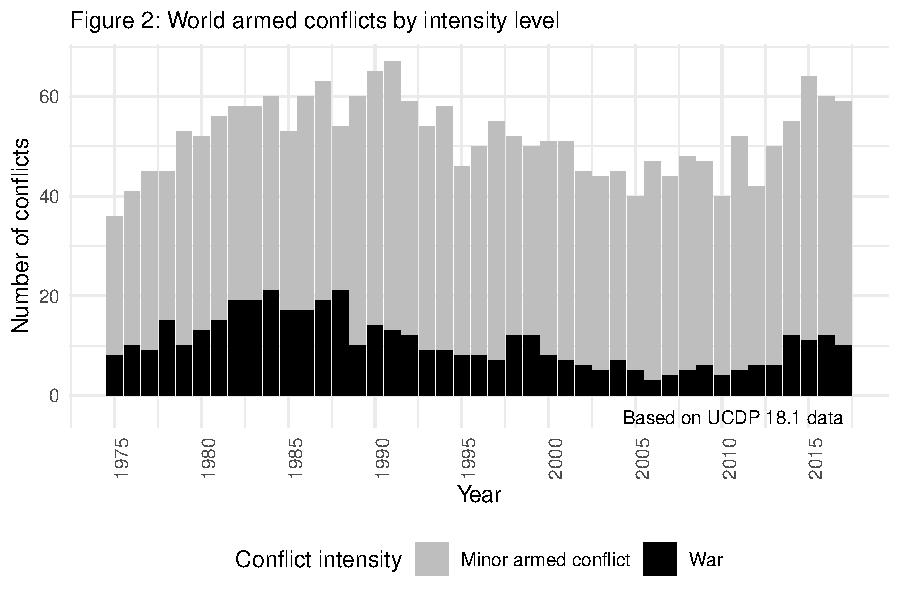
\includegraphics[keepaspectratio]{Paper_writeup_files/figure-latex/Figure 2: Intensity-1.pdf}}

While most conflicts are fought in Asia and Africa, the number of
conflicts fought in the Middle East is growing (Appendix 1), with
conflicts in Asia and the Americas portraying longer duration (Figure
3).

\pandocbounded{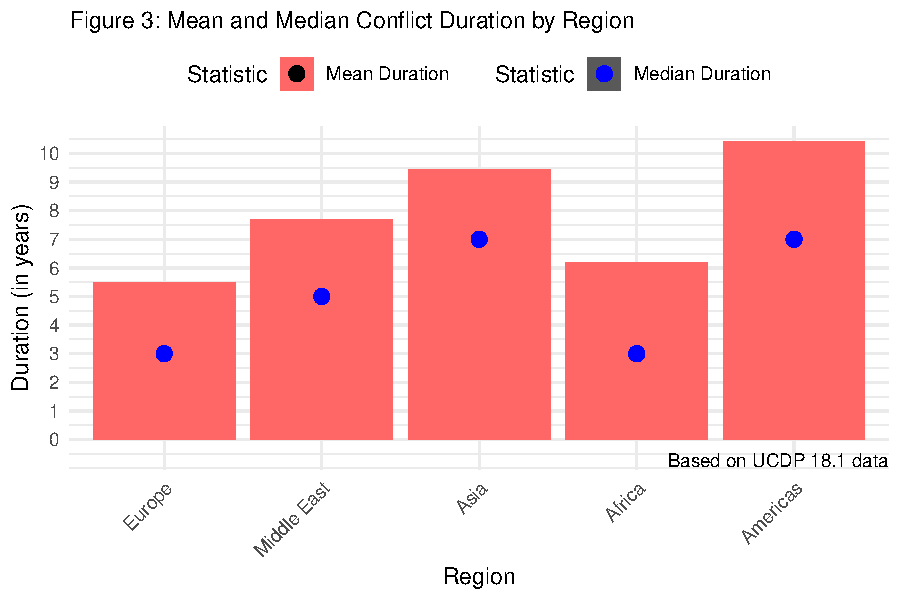
\includegraphics[keepaspectratio]{Paper_writeup_files/figure-latex/Figure 3: Duration-1.pdf}}

Intrastate conflicts are the most common type of conflict, followed by
internationalised intrastate conflicts, whose number has been growing
since the early 2000s (Appendix 2). While there is fluctuation between
the incompatibility types `territory' and `government', most conflicts
in 2017 were about territory and hardly any about territory and
government (Appendix 4).

\subsection{The provision of external
support}\label{the-provision-of-external-support}

The provision of ES has risen, with indirect support being the most
common (Figure 4) and supporters providing three forms of support on
average (Median: 4). The provision of support in a coalition has
increased over time (Appendix 5).

\pandocbounded{
\includegraphics[keepaspectratio]{Paper_writeup_files/figure-latex/Figure 4 (In-)direct support-1.pdf}}

The model for the provision of ES (Table 2) shows no statistically
significant results. However, the results of the regression analyses for
individual forms of support reveal distinct patterns in the relationship
between conflict characteristics and the provision of ES, with notable
differences between within and between models.

\newpage

\noindent\textbf{Table 2: Regression Results – External Support Determinants}

\begin{tabular}{ll}
\hline
& Within-between \\ \hline
(Intercept) & \num{1.004} \\
& [\num{0.862}, \num{1.170}] \\
Type (interstate) & \num{1.004} \\
& [\num{0.540}, \num{1.867}] \\
Type (internationalised intrastate) & \num{1.005} \\
& [\num{0.865}, \num{1.166}] \\
AIC & \num{2707.6} \\
BIC & \num{2785.6} \\
min\_wave & 0 \\
max\_wave & 42 \\
N & 208 \\
model & within-between \\
\hline
\end{tabular}

Table 3a and 3b reveal important differences in how conflict
characteristics correlate with the provision of various forms of ES,
both within conflicts (i.e., changes over time within the same dyad) and
between conflicts (i.e., differences across dyads). The provision of ES
is less correlated to conflict characteristics within conflicts (Table
3a) than between conflicts (Table 3b) and the effects of conflict
characteristics on the provision of ES tend to be smaller, with all
effect sizes below 15 within conflicts.

The era post-9/11, as well as conflict intensity and duration, show the
most significance across within models. However, the effect of these
characteristics on the provision of ES within conflicts is very small,
with only the effect of the 9/11 on the provision of weapons (8.06) and
the effect of conflict intensity on materiel and statistics provision
(11.11) exceeding an effect size of 5. Conflict intensity and duration
are only correlated with the provision of indirect ES but not with the
provision of direct support.

Within conflict-dyads, the provision of weapons, funding, and
intelligence are correlated with most conflict characteristics, with
conflict intensity, duration, and the post-9/11 era being significant in
all three. The provision of troop support is not correlated to any
conflict characteristics, while troop presence is only correlated to
conflict duration. Training and expertise is not correlated to any
conflict characteristics and the provision of materiel and statistics,
access to infrastructure, and access to territory are only correlated to
one or two conflict characteristics. All conflict characteristics only
show small effects (below 15 in all and below 5 in all but three cases)
on ES provision within conflict-dyads.

In the between logistic regression (Table 3b), the type of conflict ---
particularly internationalised intrastate conflicts --- and conflict
intensity emerge as strongly correlated to the provision of ES, showing
significance in six (intensity) and seven (type) of the nine models.
While the effect of conflict intensity on the provision of different
forms of ES is small to moderate (reaching from an effect of 0.15 on
access to territory to an effect of 19.09 on the provision of funding),
the effect of conflict type on ES provision ranges from small to high,
depending on the form of support. I.e., while the odds of receiving
training and expertise are only 0.29 units higher compared to intrastate
conflicts, the odds of receiving troop support are 87.72 units higher
compared to intrastate conflicts, holding all other factors constant.
Other influential factors include conflict duration, and the post-9/11
period, which are strongly correlated with multiple forms of support.
While the effect of conflict duration stays small (below 2 in all cases)
between conflict-dyads, 9/11 portrays an extremly high effect of 191.83
on intelligence provision and a high effect on access to infrastructure
(17.97) and troop support (19.69) between conflict-dyads.

Foreign troop presence, weapons, and materiel and statistics provision
appear to be the most sensitive to conflict characteristics, with three
to four out of seven independent variables reaching statistical
significance. Troop support, access to infrastructure, training and
expertise, funding, and access to territory all show correlation to two
conflict characteristics, while intelligence is only correlated to one
conflict characteristic. While not influenced by many conflict
characteristics the effects of conflict characteristics on troop support
and intelligence are the highest among all models. While troop support
is correlated to the type of conflict, troop presence is further
correlated to conflict intensity, duration and the post-9/11 period.

\begin{landscape}
\begin{table}[!h]
\centering
\caption{\label{tab:Table 3: WBM logistic and PPML regression - statistical significance}Table 3a: Statistical Significance in the Within Logistic and PPML Regression Models}
\centering
\resizebox{\ifdim\width>\linewidth\linewidth\else\width\fi}{!}{
\fontsize{8}{10}\selectfont
\begin{tabular}[t]{lccccccccc}
\toprule
Independent Variable & Troop Support & Troop Presence & Access to Infrastructure & Weapons & Materiel and Statistics & Training and Expertise & Funding & Intelligence & Access to Territory\\
\midrule
Intercept &  &  &  &  &  &  &  &  & \\
Territorial dispute &  &  &  &  &  &  &  &  & \\
Type of conflict &  &  &  &  &  &  &  &  & \\
Intensity &  &  &  & ** (War) & * (War) &  & *** (War) & ** (War) & \\
Duration &  & * &  & ** &  &  & *** & ** & \\
\addlinespace
9/11 &  &  & ** (After) & *** (After) &  &  & * (After) & * (After) & * (After)\\
Cold War &  &  &  & * (After) &  &  &  & * (After) & \\
Coalition Support &  &  & * (Coalition) &  & . (Coalition) &  & * (Coalition) &  & \\
N & 208 & 208 & 208 & 208 & 208 & 208 & 208 & 208 & 208\\
AIC & 877.15 & 282.08 & 1109.38 & 935.08 & 1046.81 & 2641.1 & 1144.73 & 823.69 & 1168.21\\
\addlinespace
BIC & 955.15 & 360.08 & 1187.37 & 1013.08 & 1124.8 & 2719.09 & 1222.72 & 901.69 & 1246.21\\
\bottomrule
\end{tabular}}
\end{table}
\vspace{1cm}
\begin{table}[!h]
\centering
\caption{\label{tab:Table 3: WBM logistic and PPML regression - statistical significance}Table 3b: Statistical Significance in the Between Logistic and PPML Regression Models}
\centering
\resizebox{\ifdim\width>\linewidth\linewidth\else\width\fi}{!}{
\fontsize{8}{10}\selectfont
\begin{tabular}[t]{lccccccccc}
\toprule
Independent Variable & Troop Support & Troop Presence & Access to Infrastructure & Weapons & Materiel and Statistics & Training and Expertise & Funding & Intelligence & Access to Territory\\
\midrule
Intercept & *** & *** & *** & *** &  & *** &  & *** & *\\
Territorial dispute &  &  &  &  &  &  &  &  & \\
Type of conflict & *** (Interstate); *** (Internationalised intrastate) & . (Internationalised intrastate) & ** (Internationalised intrastate) & . (Internationalised intrastate) & *** (Internationalised intrastate) & * (Interstate) & * (Internationalised intrastate) &  & \\
Intensity &  & ** (War) &  & ** (War) & ** (War) & * (War) & *** (War) &  & . (War)\\
Duration &  & * &  &  & * &  &  &  & *\\
\addlinespace
9/11 &  & * (After) & ** (After) &  &  &  &  & *** (After) & \\
Cold War &  &  &  & *** (After) &  &  &  &  & \\
Coalition Support &  &  &  &  &  &  &  &  & \\
N & 208 & 208 & 208 & 208 & 208 & 208 & 208 & 208 & 208\\
AIC & 877.15 & 282.08 & 1109.38 & 935.08 & 1046.81 & 2641.1 & 1144.73 & 823.69 & 1168.21\\
\addlinespace
BIC & 955.15 & 360.08 & 1187.37 & 1013.08 & 1124.8 & 2719.09 & 1222.72 & 901.69 & 1246.21\\
\bottomrule
\end{tabular}}
\end{table}
\end{landscape}

Already presented in Table 3, the models for troop support and weapons
were selected for detailed analysis to explore how different conflict
characteristics correlate with the provision of direct versus indirect
support. While both models use a within-between specification, the model
for troop support employs a PPML regression, and the model for weapons
provision uses a logistic regression.

The provision of troop support is most strongly correlated with the type
of conflict in the between model, while the provision of weapons shows
broader but more varied correlations with conflict characteristics in
both model components (Table 4). Specifically, between conflict dyads,
the IRR of receiving foreign troop support is 25.8 units higher (p
\textless{} 0.001) for interstate conflicts and 87.72 units higher (p
\textless{} 0.001) for internationalised intrastate conflicts, compared
to intrastate conflicts, holding all other variables constant. In
contrast, the between model for weapons provision finds that conflict
type is less consistently significant, with only internationalised
intrastate conflicts nearing significance and showing moderately higher
odds (odds = 2.31, p = 0.05) for weapon support, while interstate
conflicts show no significant association.

The intensity of a conflict is significantly correlated with weapons
provision in both within and between models. In the between model, wars
are associated with 13.75 higher odds (p = 0.01) of receiving weapons
than minor conflicts, and in the within model, the odds increase by 2.88
units (p = 0.01) when a conflict escalates to war, controlling for all
dyad-level variation. In contrast, conflict intensity is not
significantly correlated with troop support in either component of the
model. The duration of conflict also exhibits different patterns across
models. For weapons, the within model shows that the odds of receiving
weapons increase by 0.92 units (p = 0.01) with each additional year in a
conflict. No such within-group effect emerges in the troop support
model. In the between model, neither outcome is significantly associated
with the average duration of conflict.

Temporal conflict markers also yield divergent results. Both models
indicate that conflicts occurring after the Cold War are correlated with
the provision of weapons, but not with troop support. Controlling for
all between-dyad variation, the odds of receiving weapons increase by
0.2 units (p = 0.02) after the Cold War compared to during the war
within each dyad. In the between component of the model, conflicts with
a higher proportion of years occurring during the Cold War period were
associated with significantly lower odds of receiving weapons support
(odds = 0.04, p \textless{} 0.001). The within model for weapons
provision indicates that conflicts occurring after 9/11 are associated
with higher odds (odds = 8.06, p \textless{} 0.001) of receiving weapons
than conflicts happening before 9/11, while this effect is absent in the
between model. No comparable effect is found in the troop support model.

Neither model finds statistically significant effects for
coalition-based support or territorial incompatibility in either the
within or between components. In sum, while troop support appears to be
driven largely by structural characteristics of the conflict,
particularly its type, the provision of weapons is more responsive to
dynamic factors within conflicts, including duration, intensity, and
geopolitical shifts such as the post-9/11 context.

\noindent\textbf{Table 4: WBM Logistic Regression Results}

\begin{tabular}{lll}
\hline
& Troop Support & Weapons \\ \hline
(Intercept) & \num{0.012}*** & \num{32.442}*** \\
& [\num{0.006}, \num{0.025}] & [\num{7.042}, \num{149.461}] \\
Type (interstate) & \num{25.803}*** & \num{0.117} \\
& [\num{6.793}, \num{98.015}] & [\num{0.000}, \num{36.994}] \\
Type (internationalised intrastate) & \num{87.715}*** & \num{2.302}* \\
& [\num{45.671}, \num{168.465}] & [\num{1.015}, \num{5.221}] \\
AIC & \num{877.2} & \num{935.1} \\
BIC & \num{955.2} & \num{1013.1} \\
min\_wave & 0 & 0 \\
max\_wave & 42 & 42 \\
N & 208 & 208 \\
model & within-between & within-between \\
pR2\_fe &  & 0.202482056087455 \\
pR2\_total &  & 0.80941922226455 \\
\hline
\end{tabular}

All models were tested against standard regression assumptions to ensure
validity and reliability. UCDP data was deemed appropriate for
addressing the research questions, as it comprehensively captures AC and
ES characteristics, although empirical datasets rarely meet all
theoretical criteria perfectly (Gelman and Hill (2006)). Table 1
confirmed the functionality of the dependent variables.
Multicollinearity was assessed using VIFs, with all values below 5,
indicating no significant collinearity issues (O'Brien (2007)). As most
predictors were categorical, the linearity assumption did not apply. The
assumption of independent errors was violated due to repeated
observations per conflict and dyad. Homoscedasticity and residual
normality were not applicable to logistic models. The binary nature of
the dependent variable confirmed the appropriateness of logistic
regression for the analysis.

\section{Discussion}\label{discussion}

The findings of this study align with existing literature on conflict
dynamics and external interventions. Over time, the number of wars has
slightly increased, indicating a shift towards more intense conflicts,
while conflict duration has increased, suggesting that many conflicts
persist rather than being resolved. These trends are consistent with
research highlighting the protracted nature of modern ACs (Quinn et al.
(2007)). The nature of ES has also evolved. While troop support has
declined, the total number of external interventions continues to rise
(Figure 4), demonstrating a persistent strategic interest in shaping
conflict trajectories through both direct and indirect means (Davies et
al. (2024); Chang and Sellak (2022)). Recent years have seen a shift
toward multilateral coalitions and collaborative interventions (Appendix
5), with nearly one-third of all support instances involving such
coalitions, reflecting a greater emphasis on burden-sharing and
legitimacy (Meier et al. (2023)).

The findings from the regression analysis suggest that while structural
conflict factors are correlated to the provision of ES, temporal and
contextual elements play a decisive role within individual conflicts.
This aligns with existing literature on the provision of ES, which
emphasises the importance of conflict characteristics in shaping
external intervention strategies (Berlin and Malone (2023); Davies et
al. (2024)). While the models examining HG1 show no statistically
significant results, regression analyses for individual forms of support
reveal distinct patterns in the relationship between conflict
characteristics and the provision of ES, with notable differences in the
within and between results. The magnitude of effect sizes across models
contributes an additional layer to these findings, complementing
statistical significance and offering insights into the substantive
impact of various predictors.

The relatively small effects of conflict characteristics on ES provision
within conflict-dyads suggest that although factors such as duration,
conflict intensity, and the post-9/11 period are statistically
significant in some models, their practical influence on the provision
of ES within dyads may be modest. Exceptions include the post-9/11
period's effect on weapons provision, and conflict intensity's effect on
the provision of materiel and statistics, indicating a heightened
responsiveness of certain forms of indirect support to geopolitical
shifts. The larger and more variable effect sizes, especially for the
type of conflict and temporal markers between conflict-dyads suggest
that conflict type is a key driver of direct military engagement across
conflict contexts.

While troop support displays high odds ratios in the between model, it
is only significantly associated with conflict type, suggesting a narrow
but powerful predictor. Conversely, access to infrastructure, weapons,
and materiel and statistics --- forms of indirect support --- show
broader sensitivity to multiple conflict characteristics and are often
accompanied by moderate effect sizes. This pattern reinforces findings
from existing scholarship which argues that indirect ES is increasingly
favoured in modern interventions due to its strategic flexibility and
lower political cost (Meier et al. (2023); Berlin and Malone (2023)).
While no trends could be discovered in the provision of direct forms of
support and the correlation to different conflict characteristics of
troop presence and troop support might seem counter intuitive at first,
it could indicate an escalation in the provision of ES with the former
being a precondition for the latter. Conflict intensity, the post-9/11
period, conflict type (between) and conflict duration (within and
between) might be first incentives for external supporters to provide
more direct support but once troops are already present, the type of
conflict might then become a more important factor in the decision to
provide troop support. Therefore, HG1 cannot be completely rejected but
the results rather indicate that the provision of ES is not only
correlated to conflict characteristics but that it may further be
dependent on the form of support provided.

For HG2, which explores whether conflict characteristics influence the
type of ES provided, results reveal that conflict intensity (H2a) is
significantly correlated to the provision of weapons, materiel and
statistics, and funding in both within and between models, as well as to
troop presence, training and expertise, intelligence, and access to
territory in either within or between conflict-dyads, albeit with
variying effect sizes. This aligns with the argument that
higher-intensity conflicts are more likely to receive ES due to concerns
about spillover effects and escalation (Cunningham (2010); Gregory
(2000)). However, intensity does not appear to significantly impact the
provision of troop support, suggesting that external actors may not
relate the intensity of a conflict to increased levels of direct
support.

Besides intensity, conflict duration (H2c) appears as strongly
correlated to the provision of weapons, funding, intelligence, and troop
presence within a conflict-dyad, and to troop presence, the provision of
materiel and statistics and access to territory between conflict-dyads.
While correlated to the provision of several forms of ES, the effect of
duration remains small in all models. The period after 9/11 (H2e) is
correlated to the provision of multiple forms of indirect support ---
particularly access to infrastructure, weapons, funding, intelligence,
and access to territory --- within conflicts, and to troop presence,
access to infrastructure and intelligence in the between results. The
striking between-model effects of the post-9/11 period's influence on
intelligence provision and access to infrastructure underlinine the
substantial shift in intervention strategies after this geopolitical
turning point. These high-magnitude effects illustrate that temporal
context can sometimes outweigh even structural characteristics,
especially in shaping forms of support associated with intelligence, and
logistical facilitation. The Cold War period (H2f) is correlated to the
provision of weapons and intelligence within conflicts and to weapons
across conflicts. These findings are consistent with research
highlighting the geopolitical significance of the Cold War and post-9/11
eras, during which intervention strategies shifted from ideological
proxy wars to more targeted and strategic forms of engagement (Testerman
(2015); Kalyvas and Balcells (2010) in Roberts (2019)). The type of
conflict (H2d) --- particularly internationalised intrastate and
interstate conflicts --- is significantly correlated with ES in the
between models, specifically troop support, troop presence, access to
infrastructure, weapons, materiel and statistics, training and
expertise, and funding. On the other hand, territorial incompatibility
(H2b) is not significantly correlated with the provision of any ES,
suggesting that this factor plays a less prominent role in shaping
external intervention strategies. The lack of significant correlations
between territorial incompatibility with ES provision is surprising, as
previous research has highlighted the importance of this factor in
shaping conflict dynamics and external interventions (Cunningham (2010);
Gregory (2000)).

Findings suggest that coalition support (H3) is significantly correlated
to access to infrastructure, materiel and statistics, and funding within
conflict-dyads. However, between conflict-dyads, it shows no statistical
significance at all. Coalition support further only yields modest
effects, suggesting that coalitional dynamics influence tactical
decisions within specific conflicts more than strategic choices across
conflicts.

Model-specific results further illustrate these patterns: troop support
is most strongly correlated to the type of conflict, whereas the
provision of weapons shows broader but less consistent correlations with
conflict characteristics. The results suggest that the type of conflict
could be a significant factor in determining the provision of troop
support between conflicts, with interstate and internationalised
intrastate conflicts being more likely to receive this form of support
than intrastate conflicts. The significance of especially
internationalised intrastate conflicts might be explained by the fact
that they are often more complex and involve multiple actors, which
creates opportunities for external actors to provide support to one side
or another, depending on their interests and objectives. The findings
highlight key theoretical implications for Criminology and conflict
studies. The weak correlation between direct support and conflict
characteristics suggests that direct military interventions may be
driven by factors beyond conflict characteristics alone, such as
diplomatic or geopolitical considerations. While statistical
significance flags robust relationships, the size of these effects
clarifies their substantive impact. The findings suggest that some
conflict characteristics exert strong influences on particular forms of
support --- notably conflict type on troop support and post-9/11 on
intelligence --- while others like territorial incompatibility show
little predictive power despite theoretical expectations. For
researchers and policymakers, this highlights the importance of not only
identifying which variables matter but also understanding how much they
matter, ensuring that theoretical claims are grounded in both
statistical and substantive relevance. The significance of temporal
markers and conflict characteristics across both dimensions suggests
that the dynamics shaping ES are multifaceted and vary depending on the
form of assistance.

The inability to control for regional variation or geographic proximity
limits the generalisability of the findings, as well as their
interpretation from a criminological perspective. Tobler (1970) law,
`everything is related to everything else, but near things are more
related than distant things' suggests that geographic proximity may play
a significant role in shaping the dynamics of ES. Not controlling for
geographic proximity might thereby ignore important contextual factors
that influence the provision of ES. Despite this, the results confirm
existing theories that ES provision is influenced by conflict
characteristics --- particularly intensity and duration --- yet also
underscore that different forms of support respond to these
characteristics in distinct ways. This supports a `cold logic'
interpretation, in which state actors rationally assess the strategic
value of conflict before engaging, rather than reacting emotionally.
This aligns with prior research suggesting intervention decisions are
based on a rational assessment of costs, benefits, and political
alignment (Schultz (2010); Bapat (2012); Sawyer et al. (2015)). However,
the absence of data on shared cultural ties or geographic proximity
prevents assessment of whether certain interventions also follow a `hot'
logic, where emotional or identity-driven factors --- such as shared
ethnicity or history --- play a role. This opens an important avenue for
future research that more explicitly incorporates emotional, symbolic,
and identity-based motivations.

Further limitations arise from the dataset's focus on state-based
conflicts, which omits the growing influence of non-state actors and
transnational networks in modern conflict. Additionally, provider and
recipient characteristics --- key to understanding the criminological
dynamics of power, ideology, and legitimacy --- could not be tested due
to data constraints. Reverse causality also poses a risk: rather than
resolving conflict, ES may prolong it by altering the incentives for
continued violence (Fearon (2004) in Testerman (2015); Lacina (2006)).
While model refitting and variable exclusion (i.e., 9/11 in the FE model
for foreign troop presence) were necessary to achieve convergence, these
changes limit comparability across models. The exclusive use of
quantitative methods further restricts insight into the lived
experiences and micro-level effects of ES. Future research should
therefore enhance this study by incorporating qualitative data and case
studies to provide a more comprehensive understanding of the
relationship between ES and conflict dynamics.

\section{Conclusion}\label{conclusion}

This study set out to examine how characteristics of AC shape the
provision of ES, offering new insights into the strategic logic
underlying state interventions. Contemporary examples such as Russia's
invasion of Ukraine, evidence the limitations of pacifist responses. But
while military interventions can at times stabilise volatile regions,
they often risk escalating violence or prolonging conflict (Fearon
(2004) in Testerman (2015); Lacina (2006); Olson Lounsbery (2016)). The
findings show that ES---particularly indirect forms---is significantly
associated with conflict characteristics, potentially suggesting a
calculated, `cold' approach to intervention. Rather than being random or
purely humanitarian, ES would then reflect strategic assessments of
conflict dynamics, reinforcing existing literature on the instrumental
use of support in warfare (Schultz (2010); Bapat (2012); Sawyer et al.
(2015)). Crucially, the type of support provided varies with conflict
characteristics, indicating that ES is not a one-size-fits-all strategy.
These results have important implications for criminology. If states
make informed, strategic decisions to intervene in armed conflicts, they
may bear greater responsibility for the violence and crimes that unfold
in these contexts. Yet, this dimension of liability and complicity
remains underexplored in criminological research. This study offers a
starting point for engaging with ES as a site of criminological concern,
where questions of accountability, harm, and power intersect. By
broadening its focus to include the indirect consequences of state
interventions, criminology can contribute to more effective policy
responses and a deeper understanding of the global production and
regulation of violence.

\section{Appendices}\label{appendices}

\pandocbounded{
\includegraphics[keepaspectratio]{Paper_writeup_files/figure-latex/Region (Appendix 1)-1.pdf}}

\pandocbounded{
\includegraphics[keepaspectratio]{Paper_writeup_files/figure-latex/Conflict type (Appendix 2)-1.pdf}}

\pandocbounded{
\includegraphics[keepaspectratio]{Paper_writeup_files/figure-latex/Bivariate analysis between conflict type and region (Appendix 3)-1.pdf}}

\pandocbounded{
\includegraphics[keepaspectratio]{Paper_writeup_files/figure-latex/Incompatibility (Appendix 4)-1.pdf}}

\pandocbounded{
\includegraphics[keepaspectratio]{Paper_writeup_files/figure-latex/Coalition Support (Appendix 5)-1.pdf}}

\section*{References}\label{references}
\addcontentsline{toc}{section}{References}

\phantomsection\label{refs}
\begin{CSLReferences}{0}{1}
\bibitem[\citeproctext]{ref-AbrahmsMax2018ECAT}
Abrahms, M., Ward, M. and Kennedy, R. (2018). Explaining civilian
attacks: Terrorist networks, principal-agent problems and target
selection. \emph{Perspectives on terrorism (Lowell)}, 12(1), pp.23--45.
{[}online{]}. Available from:
\url{https://www.jstor.org/stable/26343744} {[}Accessed April 21,
2025{]}.

\bibitem[\citeproctext]{ref-AndersonNoel2019CIPC}
Anderson, N. (2019).
\href{https://doi.org/10.1093/isq/sqz037}{Competitive intervention,
protracted conflict, and the global prevalence of civil war}.
\emph{International studies quarterly}, 63(3), pp.692--706.

\bibitem[\citeproctext]{ref-AydinAysegul2012Noti}
Aydin, A. and Regan, P.M. (2012).
\href{https://doi.org/10.1177/1354066111403515}{Networks of third-party
interveners and civil war duration}. \emph{European journal of
international relations}, 18(3), pp.573--597.

\bibitem[\citeproctext]{ref-BaconTricia2018ItEo}
Bacon, T. (2018).
\href{https://doi.org/10.1080/09636412.2017.1416813}{Is the enemy of my
enemy my friend?: How terrorist groups select partners}. \emph{Security
studies}, 27(3), pp.345--378.

\bibitem[\citeproctext]{ref-Balch-LindsayDylan2008TIat}
Balch-Lindsay, D., Enterline, A.J. and Joyce, K.A. (2008).
\href{https://doi.org/10.1177/0022343308088815}{Third-party intervention
and the civil war process}. \emph{Journal of peace research}, 45(3),
pp.345--363.

\bibitem[\citeproctext]{ref-BapatNavinA.2012USSo}
Bapat, N.A. (2012).
\href{https://doi.org/10.1017/S000712341100007X}{Understanding state
sponsorship of militant groups}. \emph{British journal of political
science}, 42(1), pp.1--29.

\bibitem[\citeproctext]{ref-BenjaminDanielJ.2018Rss}
Benjamin, D.J. et al. (2018).
\href{https://doi.org/10.1038/s41562-017-0189-z}{Redefine statistical
significance}. \emph{Nature human behaviour}, 2(1), pp.6--10.

\bibitem[\citeproctext]{ref-BerlinMark2023GamH}
Berlin, M. and Malone, I. (2023).
\href{https://doi.org/10.1080/03050629.2023.2201881}{Go arm me: How
militant fragmentation affects external support}. \emph{International
interactions}, 49(4), pp.557--586.

\bibitem[\citeproctext]{ref-BhattaraiPrakash2016Tcic}
Bhattarai, P. (2016).
\href{https://doi.org/10.1108/IJCMA-08-2014-0066}{Third-party
coordination in conflict resolution: Evidence from nepal and the
philippines}. \emph{The International journal of conflict management},
27(3), pp.398--423.

\bibitem[\citeproctext]{ref-ChangYang-Ming2022Atoc}
Chang, Y.-M. and Sellak, M. (2022).
\href{https://doi.org/10.1080/00036846.2021.2016588}{A theory of
competing interventions by external powers in intrastate conflicts:
Implications for war and armed peace}. \emph{Applied economics}, 54(33),
pp.3811--3822.

\bibitem[\citeproctext]{ref-collins2008}
Collins, R. (2008). \emph{Violence : A micro-sociological theory /
randall collins.} Princeton, N.J. ; Princeton University Press.

\bibitem[\citeproctext]{ref-correia2020ppmlhdfe}
Correia, S., Guimarães, P. and Zylkin, T. (2020). Fast poisson
estimation with high-dimensional fixed effects. \emph{The Stata
Journal}, 20(1), pp.95--115. {[}online{]}. Available from:
\url{https://doi.org/10.1177/1536867X20909691}.

\bibitem[\citeproctext]{ref-CunninghamDavidE.2010BrHe}
Cunningham, D.E. (2010).
\href{https://doi.org/10.1177/0022343309353488}{Blocking resolution: How
external states can prolong civil wars}. \emph{Journal of peace
research}, 47(2), pp.115--127.

\bibitem[\citeproctext]{ref-CUNNINGHAMDAVIDE.2016PCWH}
Cunningham, D.E. (2016).
\href{https://doi.org/10.1017/S0043887115000404}{PREVENTING CIVIL WAR:
How the potential for international intervention can deter conflict
onset}. \emph{World politics}, 68(2), pp.307--340.

\bibitem[\citeproctext]{ref-DaviesShawn2024Ov1a}
Davies, S. et al. (2024).
\href{https://doi.org/10.1177/00223433241262912}{Organized violence
1989--2023, and the prevalence of organized crime groups}. \emph{Journal
of peace research}, 61(4), pp.673--693.

\bibitem[\citeproctext]{ref-FairbrotherMalcolm2014TMMT}
Fairbrother, M. (2014). \href{https://doi.org/10.1017/psrm.2013.24}{Two
multilevel modeling techniques for analyzing comparative longitudinal
survey datasets}. \emph{Political science research and methods}, 2(1),
pp.119--140.

\bibitem[\citeproctext]{ref-FangXiangming2020TECo}
Fang, X. et al. (2020).
\href{https://doi.org/10.5089/9781513559667.001}{The economic
consequences of conflict in sub-saharan africa}. \emph{IMF working
paper}, 20(221).

\bibitem[\citeproctext]{ref-federle2024price}
Federle, J. et al. (2024). \emph{The price of war}. Centre for Economic
Policy Research. {[}online{]}. Available from:
\url{https://mutschler.eu/files/papers/Price_of_War_2024_CEPR.pdf}
{[}Accessed April 21, 2025{]}.

\bibitem[\citeproctext]{ref-FindleyMichaelG.2006RTIi}
Findley, M.G. and Teo, T.K. (2006).
\href{https://doi.org/10.1111/j.1468-2508.2006.00473.x}{Rethinking
third-party interventions into civil wars: An actor-centric approach}.
\emph{The Journal of politics}, 68(4), pp.828--837.

\bibitem[\citeproctext]{ref-FleischerNL2008Udag}
Fleischer, N.L. and Diez Roux, A.V. (2008).
\href{https://doi.org/10.1136/jech.2007.067371}{Using directed acyclic
graphs to guide analyses of neighbourhood health effects: An
introduction}. \emph{Journal of epidemiology and community health
(1979)}, 62(9), pp.842--846.

\bibitem[\citeproctext]{ref-Gelman_Hill_2006}
Gelman, A. and Hill, J. (2006). \emph{Data analysis using regression and
multilevel/hierarchical models}. Cambridge University Press.

\bibitem[\citeproctext]{ref-GleditschKristianSkrede2007TDoC}
Gleditsch, K.S. (2007).
\href{https://doi.org/10.1177/0022343307076637}{Transnational dimensions
of civil war}. \emph{Journal of peace research}, 44(3), pp.293--309.

\bibitem[\citeproctext]{ref-GoldmanOgenS.2016Dftr}
Goldman, O.S. and Abulof, U. (2016).
\href{https://doi.org/10.1080/13523260.2016.1228033}{Democracy for the
rescue-of dictators? The role of regime type in civil war
interventions}. \emph{Contemporary security policy}, 37(3), pp.341--368.

\bibitem[\citeproctext]{ref-GregoryShaun2000TFMI}
Gregory, S. (2000). \href{https://doi.org/10.1093/afraf/99.396.435}{THE
FRENCH MILITARY IN AFRICA: PAST AND PRESENT}. \emph{African affairs
(London)}, 99(396), pp.435--448.

\bibitem[\citeproctext]{ref-hagan2015criminology}
Hagan, J. (2015). While criminology slept: A criminal war of aggression
in iraq. \emph{The Criminologist: The Official Newsletter of the
American Society of Criminology}, 40(6), pp.2--4. {[}online{]}.
Available from:
\url{https://asc41.org/wp-content/uploads/ASC-Criminologist-2015-11.pdf}
{[}Accessed April 21, 2025{]}.

\bibitem[\citeproctext]{ref-HarbomLotta2008DDoA}
Harbom, L., Melander, E. and Wallensteen, P. (2008).
\href{https://doi.org/10.1177/0022343308094331}{Dyadic dimensions of
armed conflict, 1946-2007}. \emph{Journal of peace research}, 45(5),
pp.697--710.

\bibitem[\citeproctext]{ref-hillyardandtombs2007}
Hillyard, P. and Tombs, S. (2007).
\href{https://doi.org/10.1007/s10611-007-9079-z}{From {`crime'} to
social harm?} \emph{Crime, Law and Social Change}, 48, pp.9--25.

\bibitem[\citeproctext]{ref-hoeffler2003measuring}
Hoeffler, A. and Reynal-Querol, M. (2003). \emph{Measuring the costs of
conflict}. Centre for the Study of African Economies, University of
Oxford; The World Bank. {[}online{]}. Available from:
\url{https://v1.cepa.lk/content_images/publications/documents/1005-S-Hoeffler\%20and\%20Reynal-Measuring\%20the\%20Costs\%20of\%20Conflict.pdf}
{[}Accessed April 21, 2025{]}.

\bibitem[\citeproctext]{ref-huntingtonklein2023fixed}
Huntington-Klein, N. (2023). Fixed effects. In \emph{The effect: An
introduction to research design and causality}. CRC Press, A Chapman \&
Hall Book. {[}online{]}. Available from:
\url{https://theeffectbook.net/ch-FixedEffects.html}.

\bibitem[\citeproctext]{ref-doi:10.1177ux2f13624806030073001}
Jamieson, R. (2003). Introduction. \emph{Theoretical Criminology}, 7(3),
pp.259--263. {[}online{]}. Available from:
\url{https://doi.org/10.1177/13624806030073001}.

\bibitem[\citeproctext]{ref-Karluxe9nNiklas2023EtDE}
Karlén, N. (2023).
\href{https://doi.org/10.1080/1057610X.2020.1835002}{Escalate to
de-escalate? External state support and governments' willingness to
negotiate}. \emph{Studies in conflict and terrorism}, 46(8),
pp.1323--1344.

\bibitem[\citeproctext]{ref-Karluxe9nNiklas2017Tlof}
Karlén, N. (2017). \href{https://doi.org/10.1177/0022343317700465}{The
legacy of foreign patrons: External state support and conflict
recurrence}. \emph{Journal of peace research}, 54(4), pp.499--512.

\bibitem[\citeproctext]{ref-Karluxe9nNiklas2019TotT}
Karlén, N. (2019).
\href{https://doi.org/10.1080/09546553.2017.1282861}{Turning off the
taps: The termination of state sponsorship}. \emph{Terrorism and
political violence}, 31(4), pp.733--758.

\bibitem[\citeproctext]{ref-KathmanJacobD.2011CWDa}
Kathman, J.D. (2011).
\href{https://doi.org/10.1177/0022002711408009}{Civil war diffusion and
regional motivations for intervention}. \emph{Journal of Conflict
Resolution}, 55(6), pp.847--876.

\bibitem[\citeproctext]{ref-KleinJoshR2011Tacc}
Klein, J.R. (2011). Toward a cultural criminology of war. \emph{Social
justice (San Francisco, Calif.)}, 38(3), pp.86--103. {[}online{]}.
Available from: \url{https://www.jstor.org/stable/41940949} {[}Accessed
February 13, 2025{]}.

\bibitem[\citeproctext]{ref-KramerRonaldC.2005WAAS}
Kramer, R.C. and Michalowski, R.J. (2005).
\href{https://doi.org/10.1093/bjc/azi032}{WAR, AGGRESSION AND STATE
CRIME: A criminological analysis of the invasion and occupation of
iraq}. \emph{British journal of criminology}, 45(4), pp.446--469.

\bibitem[\citeproctext]{ref-LacinaBethany2006EtSo}
Lacina, B. (2006).
\href{https://doi.org/10.1177/0022002705284828}{Explaining the severity
of civil wars}. \emph{The Journal of conflict resolution}, 50(2),
pp.276--289.

\bibitem[\citeproctext]{ref-LeThai-Ha2022Easi}
Le, T.-H., Bui, M.-T. and Uddin, G.S. (2022).
\href{https://doi.org/10.1016/j.econmod.2022.105980}{Economic and social
impacts of conflict: A cross-country analysis}. \emph{Economic
modelling}, 115, pp.105980--.

\bibitem[\citeproctext]{ref-MaozZeev2012RaSS}
Maoz, Z. and San-Akca, B. (2012).
\href{https://doi.org/10.1111/j.1468-2478.2012.00759.x}{Rivalry and
state support of non-state armed groups (NAGs), 1946-2001 1: Rivalry and
state support of non-state armed groups}. \emph{International studies
quarterly}, 56(4), pp.720--734.

\bibitem[\citeproctext]{ref-McGarryRoss2016IToW}
McGarry, R. et al. (2016).
\href{https://doi.org/10.1057/978-1-137-43170-7_1}{Introduction: The
criminology of war, what is it good for?} In \emph{The palgrave handbook
of criminology and war}. United Kingdom: Palgrave Macmillan UK, pp.
1--21.

\bibitem[\citeproctext]{ref-McGarryRoss2019ICtb}
McGarry, R. and Walklate, S. (2019).
\href{https://doi.org/10.51952/9781529202618.ch001}{Introduction: Can
there be a 'criminology of war'?} In \emph{A criminology of war?} New
horizons in criminology. Bristol, UK: Bristol University Press, pp.
1--14.

\bibitem[\citeproctext]{ref-mcgarry2015introduction}
McGarry, R. and Walklate, S. (2015). Introduction: Placing war within
criminology. In S. Walklate \& R. McGarry, eds. \emph{Criminology and
war: Transgressing the borders}. Abingdon: Routledge. {[}online{]}.
Available from:
\url{https://www.taylorfrancis.com/chapters/edit/10.4324/9781315858425-1/introduction-ross-mcgarry-sandra-walklate?context=ubx&refId=6b6a1a3e-4b01-4767-8838-da05005a9a2e}
{[}Accessed April 21, 2025{]}.

\bibitem[\citeproctext]{ref-MeierVanessa2023Esia}
Meier, V. et al. (2023).
\href{https://doi.org/10.1177/00223433221079864}{External support in
armed conflicts: Introducing the UCDP external support dataset (ESD),
1975--2017}. \emph{Journal of peace research}, 60(3), pp.545--554.

\bibitem[\citeproctext]{ref-Meier2022}
Meier, V. (2022). UCDP external support dataset (ESD) codebook v18.1.

\bibitem[\citeproctext]{ref-MeulewaeterChlouxe92021Meat}
Meulewaeter, C. (2021).
\href{https://doi.org/10.4324/9781003045823-3}{Military expenditure,
arms transfer and armed conflicts}. In J. C. Rufanges, ed.
\emph{Military spending and global security}. United Kingdom: Routledge,
pp. 22--40.

\bibitem[\citeproctext]{ref-MundlakYair1978Otpo}
Mundlak, Y. (1978). \href{https://doi.org/10.2307/1913646}{On the
pooling of time series and cross section data}. \emph{Econometrica},
46(1), pp.69--85.

\bibitem[\citeproctext]{ref-OBRIENRobertM2007Acrr}
O'Brien, R.M. (2007). \href{https://doi.org/10.1007/s11135-006-9018-6}{A
caution regarding rules of thumb for variance inflation factors}.
\emph{Quality \& quantity}, 41(5), pp.673--690.

\bibitem[\citeproctext]{ref-OlsonLounsberyMarie2016FMIP}
Olson Lounsbery, M. (2016).
\href{https://doi.org/10.1093/jogss/ogw004}{Foreign military
intervention, power dynamics, and rebel group cohesion}. \emph{Journal
of global security studies}, 1(2), pp.127--141.

\bibitem[\citeproctext]{ref-PetrovaMarinaG.2019WMIW}
Petrova, M.G. (2019).
\href{https://doi.org/10.1177/0022002719826645}{What matters is who
supports you: Diaspora and foreign states as external supporters and
militants' adoption of nonviolence}. \emph{The Journal of conflict
resolution}, 63(9), pp.2155--2179.

\bibitem[\citeproctext]{ref-PetterssonTheruxe9se2018Ov1}
Pettersson, T. and Eck, K. (2018).
\href{https://doi.org/10.1177/0022343318784101}{Organized violence,
1989--2017}. \emph{Journal of peace research}, 55(4), pp.535--547.

\bibitem[\citeproctext]{ref-PhillipsBrianJ.2019TGRa}
Phillips, B.J. (2019).
\href{https://doi.org/10.1080/1057610X.2018.1431365}{Terrorist group
rivalries and alliances: Testing competing explanations}. \emph{Studies
in conflict and terrorism}, 42(11), pp.997--1019.

\bibitem[\citeproctext]{ref-QuinnJ.Michael2007StPD}
Quinn, J.M., Mason, T.D. and Gurses, M. (2007).
\href{https://doi.org/10.1080/03050620701277673}{Sustaining the peace:
Determinants of civil war recurrence}. \emph{International
interactions}, 33(2), pp.167--193.

\bibitem[\citeproctext]{ref-R2025}
R Core Team. (2025). R: The r project for statistical computing.

\bibitem[\citeproctext]{ref-alma992976076122201631}
Rafter, N.H. (2016). \emph{The crime of all crimes: Toward a criminology
of genocide}. New York: New York University Press.

\bibitem[\citeproctext]{ref-RauchhausRobertW.2009PPiH}
Rauchhaus, R.W. (2009).
\href{https://doi.org/10.1111/j.1468-2478.2009.00560.x}{Principal-agent
problems in humanitarian intervention: Moral hazards, adverse selection,
and the commitment dilemma}. \emph{International studies quarterly},
53(4), pp.871--884.

\bibitem[\citeproctext]{ref-ReganPatrickM.1998CtIO}
Regan, P.M. (1998). \href{https://doi.org/10.2307/2647647}{Choosing to
intervene: Outside interventions in internal conflicts}. \emph{The
Journal of politics}, 60(3), pp.754--779.

\bibitem[\citeproctext]{ref-regan2002third}
Regan, P.M. (2002).
\href{https://doi.org/10.1177/0022002702046001004}{Third-party
interventions and the duration of intrastate conflicts}. \emph{Journal
of Conflict Resolution}, 46(1), pp.55--73.

\bibitem[\citeproctext]{ref-ReganPatrickM2014Doid}
Regan, P.M. and Meachum, M.S. (2014).
\href{https://doi.org/10.1177/0022343313505303}{Data on interventions
during periods of political instability}. \emph{Journal of peace
research}, 51(1), pp.127--135.

\bibitem[\citeproctext]{ref-RobertsJordan2019TaRR}
Roberts, J. (2019).
\href{https://doi.org/10.1080/13698249.2019.1648631}{Targeting and
resistance: Reassessing the effect of external support on the duration
and outcome of armed conflict}. \emph{Civil wars}, 21(3), pp.362--384.

\bibitem[\citeproctext]{ref-RuggieroVincenzo2005CWCa}
Ruggiero, V. (2005).
\href{https://doi.org/10.1177/0964663905051221}{Criminalizing war:
Criminology as ceasefire}. \emph{Social \& legal studies}, 14(2),
pp.239--257.

\bibitem[\citeproctext]{ref-RuggieroVincenzo2023Caw}
Ruggiero, V. (2023). \href{https://doi.org/10.1332/TGBW8348}{Criminology
against war}. \emph{Justice, Power and Resistance}, 6(3), pp.263--277.

\bibitem[\citeproctext]{ref-ruggiero2015achilles}
Ruggiero, V. (2015). War and the death of achilles. In S. Walklate \& R.
McGarry, eds. \emph{Criminology and war}. Routledge, pp. 21--37.

\bibitem[\citeproctext]{ref-SaidemanStephenM.2002DiIR}
Saideman, S.M. (2002).
\href{https://doi.org/10.1177/0022343302039001002}{Discrimination in
international relations: Analyzing external support for ethnic groups}.
\emph{Journal of peace research}, 39(1), pp.27--50.

\bibitem[\citeproctext]{ref-SalehyanIdean2010TDoW}
Salehyan, I. (2010). \href{https://doi.org/10.1177/0022002709357890}{The
delegation of war to rebel organizations}. \emph{The Journal of conflict
resolution}, 54(3), pp.493--515.

\bibitem[\citeproctext]{ref-SalehyanIdean2011EESf}
Salehyan, I., Gleditsch, K.S. and Cunningham, D.E. (2011).
\href{https://doi.org/10.1017/S0020818311000233}{Explaining external
support for insurgent groups}. \emph{International organization}, 65(4),
pp.709--744.

\bibitem[\citeproctext]{ref-alma992983194640301631}
San-Akca, B. (2016). \emph{States in disguise : Causes of state support
for rebel groups / belgin san-akca.} Oxford: Oxford University Press.

\bibitem[\citeproctext]{ref-CenterGlobalDevelopmentUSAIScuts}
Sandefur, J. and Kenny, C. (2025). USAID cuts: New estimates at the
country level. {[}online{]}. Available from:
\url{https://www.cgdev.org/blog/usaid-cuts-new-estimates-country-level}
{[}Accessed May 7, 2025{]}.

\bibitem[\citeproctext]{ref-SawyerKatherine2015TRoE}
Sawyer, K., Cunningham, K.G. and Reed, W. (2015).
\href{https://doi.org/10.1177/0022002715600761}{The role of external
support in civil war termination}. \emph{The Journal of conflict
resolution}, 61(6), pp.1174--1202.

\bibitem[\citeproctext]{ref-SchultzKennethA.2010TEPi}
Schultz, K.A. (2010).
\href{https://doi.org/10.1017/S0020818310000032}{The enforcement problem
in coercive bargaining: Interstate conflict over rebel support in civil
wars}. \emph{International organization}, 64(2), pp.281--312.

\bibitem[\citeproctext]{ref-SilvaJ.M.C.Santos2006TLoG}
Silva, J.M.C.S. and Tenreyro, S. (2006). The log of gravity. \emph{The
review of economics and statistics}, 88(4), pp.641--658. {[}online{]}.
Available from: \url{https://www.jstor.org/stable/40043025}.

\bibitem[\citeproctext]{ref-sivard1996world}
Sivard, R.L. (1996). \emph{World military and social expenditures}. 16th
ed. Washington, D.C., USA: World Priorities. {[}online{]}. Available
from:
\url{https://www.dropbox.com/s/wm76wylpwo5d851/WMSE\%201996\%20ed.\%20\%2816th\%29\%20by\%20Ruth\%20Sivard\%20_300dpi.pdf?dl=0}
{[}Accessed April 21, 2025{]}.

\bibitem[\citeproctext]{ref-SozerBrendan2016Dopr}
Sozer, B. (2016).
\href{https://doi.org/10.1080/09592318.2016.1189495}{Development of
proxy relationships: A case study of the lebanese civil war}.
\emph{Small wars \& insurgencies}, 27(4), pp.636--658.

\bibitem[\citeproctext]{ref-SykesGreshamM.1957ToNA}
Sykes, G.M. and Matza, D. (1957).
\href{https://doi.org/10.2307/2089195}{Techniques of neutralization: A
theory of delinquency}. \emph{American sociological review}, 22(6),
pp.664--670.

\bibitem[\citeproctext]{ref-TestermanMatthew2015RtCE}
Testerman, M. (2015).
\href{https://doi.org/10.1080/1057610X.2015.1016312}{Removing the
crutch: External support and the dynamics of armed conflict}.
\emph{Studies in conflict and terrorism}, 38(7), pp.529--542.

\bibitem[\citeproctext]{ref-Themner2018}
Themnér, L. (2018). UCDP dyadic dataset codebook, version 18.1.

\bibitem[\citeproctext]{ref-ToblerW.R.1970ACMS}
Tobler, W.R. (1970). \href{https://doi.org/10.2307/143141}{A computer
movie simulating urban growth in the detroit region}. \emph{Economic
geography}, 46, pp.234--240.

\bibitem[\citeproctext]{ref-TokdemirEfe2021RRat}
Tokdemir, E. et al. (2021).
\href{https://doi.org/10.1177/0022002720967411}{Rebel rivalry and the
strategic nature of rebel group ideology and demands}. \emph{The Journal
of conflict resolution}, 65(4), pp.729--758.

\bibitem[\citeproctext]{ref-645083f0-2904-37de-bfb3-649fda2cd398}
Toukan, M. (2019). International politics by other means: External
sources of civil war. \emph{Journal of Peace Research}, 56(6), pp.pp.
812--826. {[}online{]}. Available from:
\url{https://www.jstor.org/stable/48596232} {[}Accessed April 21,
2025{]}.

\bibitem[\citeproctext]{ref-UNUSAID}
UN. (2025). US aid cuts will make world {`less healthy, less safe and
less prosperous'}: guterres. {[}online{]}. Available from:
\url{https://news.un.org/en/story/2025/02/1160646} {[}Accessed May 7,
2025{]}.

\bibitem[\citeproctext]{ref-WalklateSandra2019TwS}
Walklate, S. and McGarry, R. (2019).
\href{https://doi.org/10.51952/9781529202618.ch002}{Theorising 'war'
within sociology and criminology}. In \emph{A criminology of war?}
Policy Press, pp. 15--40.

\bibitem[\citeproctext]{ref-WalterBarbaraF.2004DCBC}
Walter, B.F. (2004).
\href{https://doi.org/10.1177/0022343304043775}{Does conflict beget
conflict? Explaining recurring civil war}. \emph{Journal of peace
research}, 41(3), pp.371--388.

\end{CSLReferences}

\end{document}
